\subsubsection{Backend Technologies}
\textbf{Go}\\
At the start of the project, a portion of the team deliberated about which
technologies to choose for the backend. Options using JavaScript such as NodeJS
or Deno with accompanying frameworks like ExpressJS or NestJS were considered,
as was Rust and its Rocket framework. They would have been excellent choices as
they are well established in the industry and tried-and-tested.

The majority of the team has development experience with JavaScript, so going
with that would have made a lot of sense. However, it was planned from the very
beginning to deploy this application on a server hosted by one of the team
members. Therefore, the usage of computing and memory resources was very
important to them, as they did not want to strain their Kubernetes cluster more
than necessary. Since NodeJS runs on the JavaScript runtime V8, which also
powers Google Chrome, our experience indicated that it would be quite resource
intensive to run. Findings by \textcite{Tanadechopon2023} confirm this.

Due to this, the team shifted towards using compiled rather than interpreted
languages, as these are generally more resource efficient. Since small
executables and low memory usage was desired, languages and frameworks that run
on virtual machines such as Java with Spring or C\# with .Net were not deemed to
be viable options. As a result, only Rust and Go were seriously considered at
this point.

Rust offers a small package size, strong memory safety, an excellent
ecosystem and build-tools. The team member that would focus on backend
development had recent experience in writing Rust code. However, Rust
development can be very tricky and time consuming. Additionally, in our
experience Rust has above average compilation times. In a project with a fixed
deadline and the expectation of rapid development, choosing Rust would have been
detrimental. The team recognised that choosing Rust would come with many
drawbacks while offering only few benefits.

This left choosing Go as the logical conclusion. A large drawback that the team
identified with Go was the missing experience in the team. Two team members had
used Go before, but they last used it a few years back. However, since Go syntax
and the languages concepts hadn't changed much since then, it was deemed
possible to quickly get up to speed, much more quickly than Rust would have
allowed. The final decision fell on using Go, as it offered small binaries,
great memory efficiency, a solid ecosystem of libraries and build-tools and a
feature-rich, built-in library for creating REST-APIs. Go also removes a lot of
the pitfalls that Rust suffers from: it has a simple and approachable syntax and
a very low-friction, high-speed development experience. This was also the
deciding factor, since it was made clear to the team that getting an MVP up and
running as quickly as possible was imperative for the project.

\textbf{PostgreSQL}\\
The plan for the MVP of Magpie set the simple goal of delivering useful data to
users. To achieve this, the data needs to be stored in a way in which it can be
efficiently accessed during operation. Since the goal of the project was to
provide a tool to professionals, data integrity at every level was an important
consideration. Additional requirements for the data storage solution were good
support for geospatial data, quick retrieval of a large number of points and
ease-of-use.

There is a plethora of database solutions available today. The team considered
the most common types: document databases like MongoDB and multi-model databases
like PostgreSQL (sometimes called RDBMS).

While document databases like MongoDB have their place in the current
development landscape, it soon became clear that SQL-based, multi-model RDBMSs
would be best suited for the job. They offer tried-and-tested performance and
reliability and they are well equipped to guarantee data integrity. But the
deciding reason was the pre-existing experience the lead developer for the
backend had with these types of databases.

After some deliberation, \textbf{PostgreSQL} was chosen as the database solution
for this project. It was combined with the PostGIS extension to add support for
geospatial data and queries. The decision was not cut and dried as most
established multi-model databases (like Oracle DB or MySQL) offer the
functionality that the requirements were asking for. However, the Kubernetes
cluster this project was going to be deployed on already had a fully configured
PostgreSQL server running on it. Making use of pre-existing infrastructure is
the obvious choice in an agile project that had the prime goal of hitting the
ground running.

\begin{listing}[htbp]
  \centering{}
  \begin{minipage}{0.85\textwidth}
  \begin{minted}{sql}
-- name: GetPointsInRadius :many
SELECT Id, LongLat::geometry, Type from points
WHERE ST_DWithin(
  LongLat::geography,
  ST_SetSRID(
    ST_MakePoint(@longitude::float, @latitude::float), 4326
  )::geography,
  @radius::float
) AND (
  @types::point_type[] IS NULL OR Type = ANY(@types::point_type[])
);
  \end{minted}
  \end{minipage}
  \caption{An example of a SQL query with annotations used by sqlc}
  \label{listing:sqlc_query_input}
\end{listing}

\textbf{sqlc}\\
In modern software development, there are two common ways for an application to
interact with a database via SQL. There is the old school way of writing raw SQL
queries, put them into prepared statements and execute them against the
database. This gives the developer very granular control over the way their
queries are structured and how they run them. But this method requires a
significant amount of work in designing and implementing a translation layer
between the database and the application. Data that the application wants to
send to the database needs to be prepared into a format the database queries
expect. Data that the application wants to retrieve from the database needs to
be parsed back into the data model that's used by the application.

\newpage{}

To make interfacing with databases easier, so called ORMs (Object Relational
Models) were developed. These are libraries that the application developer can
include. Database queries are not done in SQL, but in the same programming
language the application is written in. The ORM provides database interface
functions that take in the data in the format the application uses. To actually
retrieve any data or make any changes to the database, the ORM runs its
internally generated SQL queries on the database using a compatible driver. ORMs
provide and abstraction layer, removing the need for directly interacting with
the database and providing a data access wrapper in the main programming
language of the project. This can make it easier and quicker to develop an
application that makes use of a database, but it takes away some of the agency
that the developer has.

The team wasn't really happy with either of these solutions, so an alternative
called \textbf{sqlc} was chosen. This tool combines the freedom that using SQL gives
developers with the productivity increase that ORMs offer. sqlc flips the
typical ORM workflow on its head. This means, the developer writes standard SQL
queries and schemas, but includes sqlc directives such as the name of the query
and the multiplicity of expected results in the comments above the query (see
Listing \ref{listing:sqlc_query_input}). These files are then passed to the CLI
of sqlc. In accordance with a configuration file provided by the developer, sqlc
then automatically generates type-safe bindings for the queries that were
defined in the SQL files (\cite{sqlc_introduction}).

This approach gives the developer more control about the queries that are
executed. At the same time, it eliminates the need to write boilerplate wrapper
code for accessing the database, just like an ORM would eliminate the need to
write SQL queries. The tool treats SQL, which is a structured and typed
language, as a source of truth. It also enables developers to reuse their
queries across systems as sqlc offers code generation for multiple programming
languages like Go, Python or Typescript and databases like PostgreSQL, MySQL or
SQLite (\cite{sqlc_documentation_language_support}).

The tool respects best practices to prevent SQL injection attacks. It generates
code that only utilises constant strings and parametrised queries
(\cite{sqlc_injection}). Using this tool, the team was quickly able to
connect the backend server to the database. Eliminating the need to update the
Go code manually each time the database schema or queries changed was vital for
the backend keeping pace with the other developers.

\begin{listing}[htbp]
  \centering{}
  \begin{minipage}{0.75\textwidth}
  \begin{minted}{yaml}
      version: "2"
      sql:
      - schema: "sql/migrations"
        queries: "sql/queries_private.sql"
        engine: "postgresql"
        gen:
          go:
            package: "db"
            sql_package: "pgx/v5"
            out: "internal/db/private"
            build_tags: "private"
            emit_json_tags: true
            overrides:
              - db_type: "geometry"
                go_type:
                  import: "github.com/twpayne/go-geom"
                  pointer: true
                  type: "Point"
      - schema: "sql/migrations"
        queries: "sql/queries_public.sql"
        engine: "postgresql"
        gen:
          go:
            package: "db"
            sql_package: "pgx/v5"
            out: "internal/db/public"
            build_tags: "public"
            emit_json_tags: true
            overrides:
              - db_type: "geometry"
                go_type:
                  import: "github.com/twpayne/go-geom"
                  pointer: true
                  type: "Point"
  \end{minted}
  \end{minipage}
  \caption{An example of a sqlc configuration file with two targets with separate query inputs and type replacement}
  \label{listing:sqlc_config_file}
\end{listing}

\newpage{}

\begin{listing}[htbp]
  \centering{}
  \begin{minipage}{0.85\textwidth}
  \begin{minted}{go}
type GetPointsInRadiusParams struct {
  Longitude float64     `json:"longitude"`
  Latitude  float64     `json:"latitude"`
  Radius    float64     `json:"radius"`
  Types     []PointType `json:"types"`
}

type GetPointsInRadiusRow struct {
  ID      int64          `json:"id"`
  Longlat *go_geom.Point `json:"longlat"`
  Type    PointType      `json:"type"`
}

func (q *Queries) GetPointsInRadius(
    ctx context.Context, arg GetPointsInRadiusParams
  ) ([]GetPointsInRadiusRow, error) {
  rows, err := q.db.Query(ctx, getPointsInRadius,
    arg.Longitude,
    arg.Latitude,
    arg.Radius,
    arg.Types,
  )
  if err != nil {
    return nil, err
  }
  defer rows.Close()
  var items []GetPointsInRadiusRow
  for rows.Next() {
    var i GetPointsInRadiusRow
    if err := rows.Scan(&i.ID, &i.Longlat, &i.Type); err != nil {
      return nil, err
    }
    items = append(items, i)
  }
  if err := rows.Err(); err != nil {
    return nil, err
  }
  return items, nil
}
  \end{minted}
  \end{minipage}
  \caption{An example of a Go binding generated by sqlc from the SQL query in
  Listing \ref{listing:sqlc_query_input}}
  \label{listing:sqlc_generated_bindings}
\end{listing}

\newpage{}

\textbf{golang-migrate}\\
During the first weeks of the project, the database was defined by a simple
initialisation SQL script. This worked fine for the time and allowed all
developers to set up their local database instance easily. But once the vertical
slice was completed, the team wanted to add additional features that would
necessitate changes to the database schema. After adding the first feature, some
developers ran into issues where the version of the backend they were running
was not compatible with the schema currently deployed on their local database.

Fixing these issues was time consuming and they were likely going to reappear
after future database changes. Realising this, the team made the decision to
integrate a database migration solution to automate this tedious process and
prevent future time losses during development.

The tool used for generating Go bindings from the raw SQL, sqlc, does not offer
any migration functionality, so another solution needed to be found. The team
evaluated all options that were listed as compatible with sqlc. These were
atlas, dbmate, golang-migrate, goose, sql-migrate and tern
(\cite{sqlc_updating_database_schema}). The team was looking for a solution that
allowed the migrations to be specified in plain SQL. The solution needed to work
both as a command-line interface application as well as a Go library, as it was
deemed necessary to apply the migrations to the database automatically. A tool
that did not rely on additional configuration files would also be preferred.
Multiple options satisfied these requirements. The backend team decided to use
\textbf{golang-migrate}, due to its straightforward usage and easy integration as a
library.

At the time this decision was taken, golang-migrate also seemed like it was
being developed most actively. This has since changed and at the time of
writing, golang-migrate is the solution with the least recent update of the
options. Nonetheless, using golang-migrate, the team was able to integrate
automated database migrations into the app, eliminating the need to spend
valuable time performing manual database updates each time the schema is
changed.

The complete database development workflow for the backend server is visualised
in Figure \ref{fig:database_workflow_diagram}.

\begin{figure}[htbp]
  \centering{}
  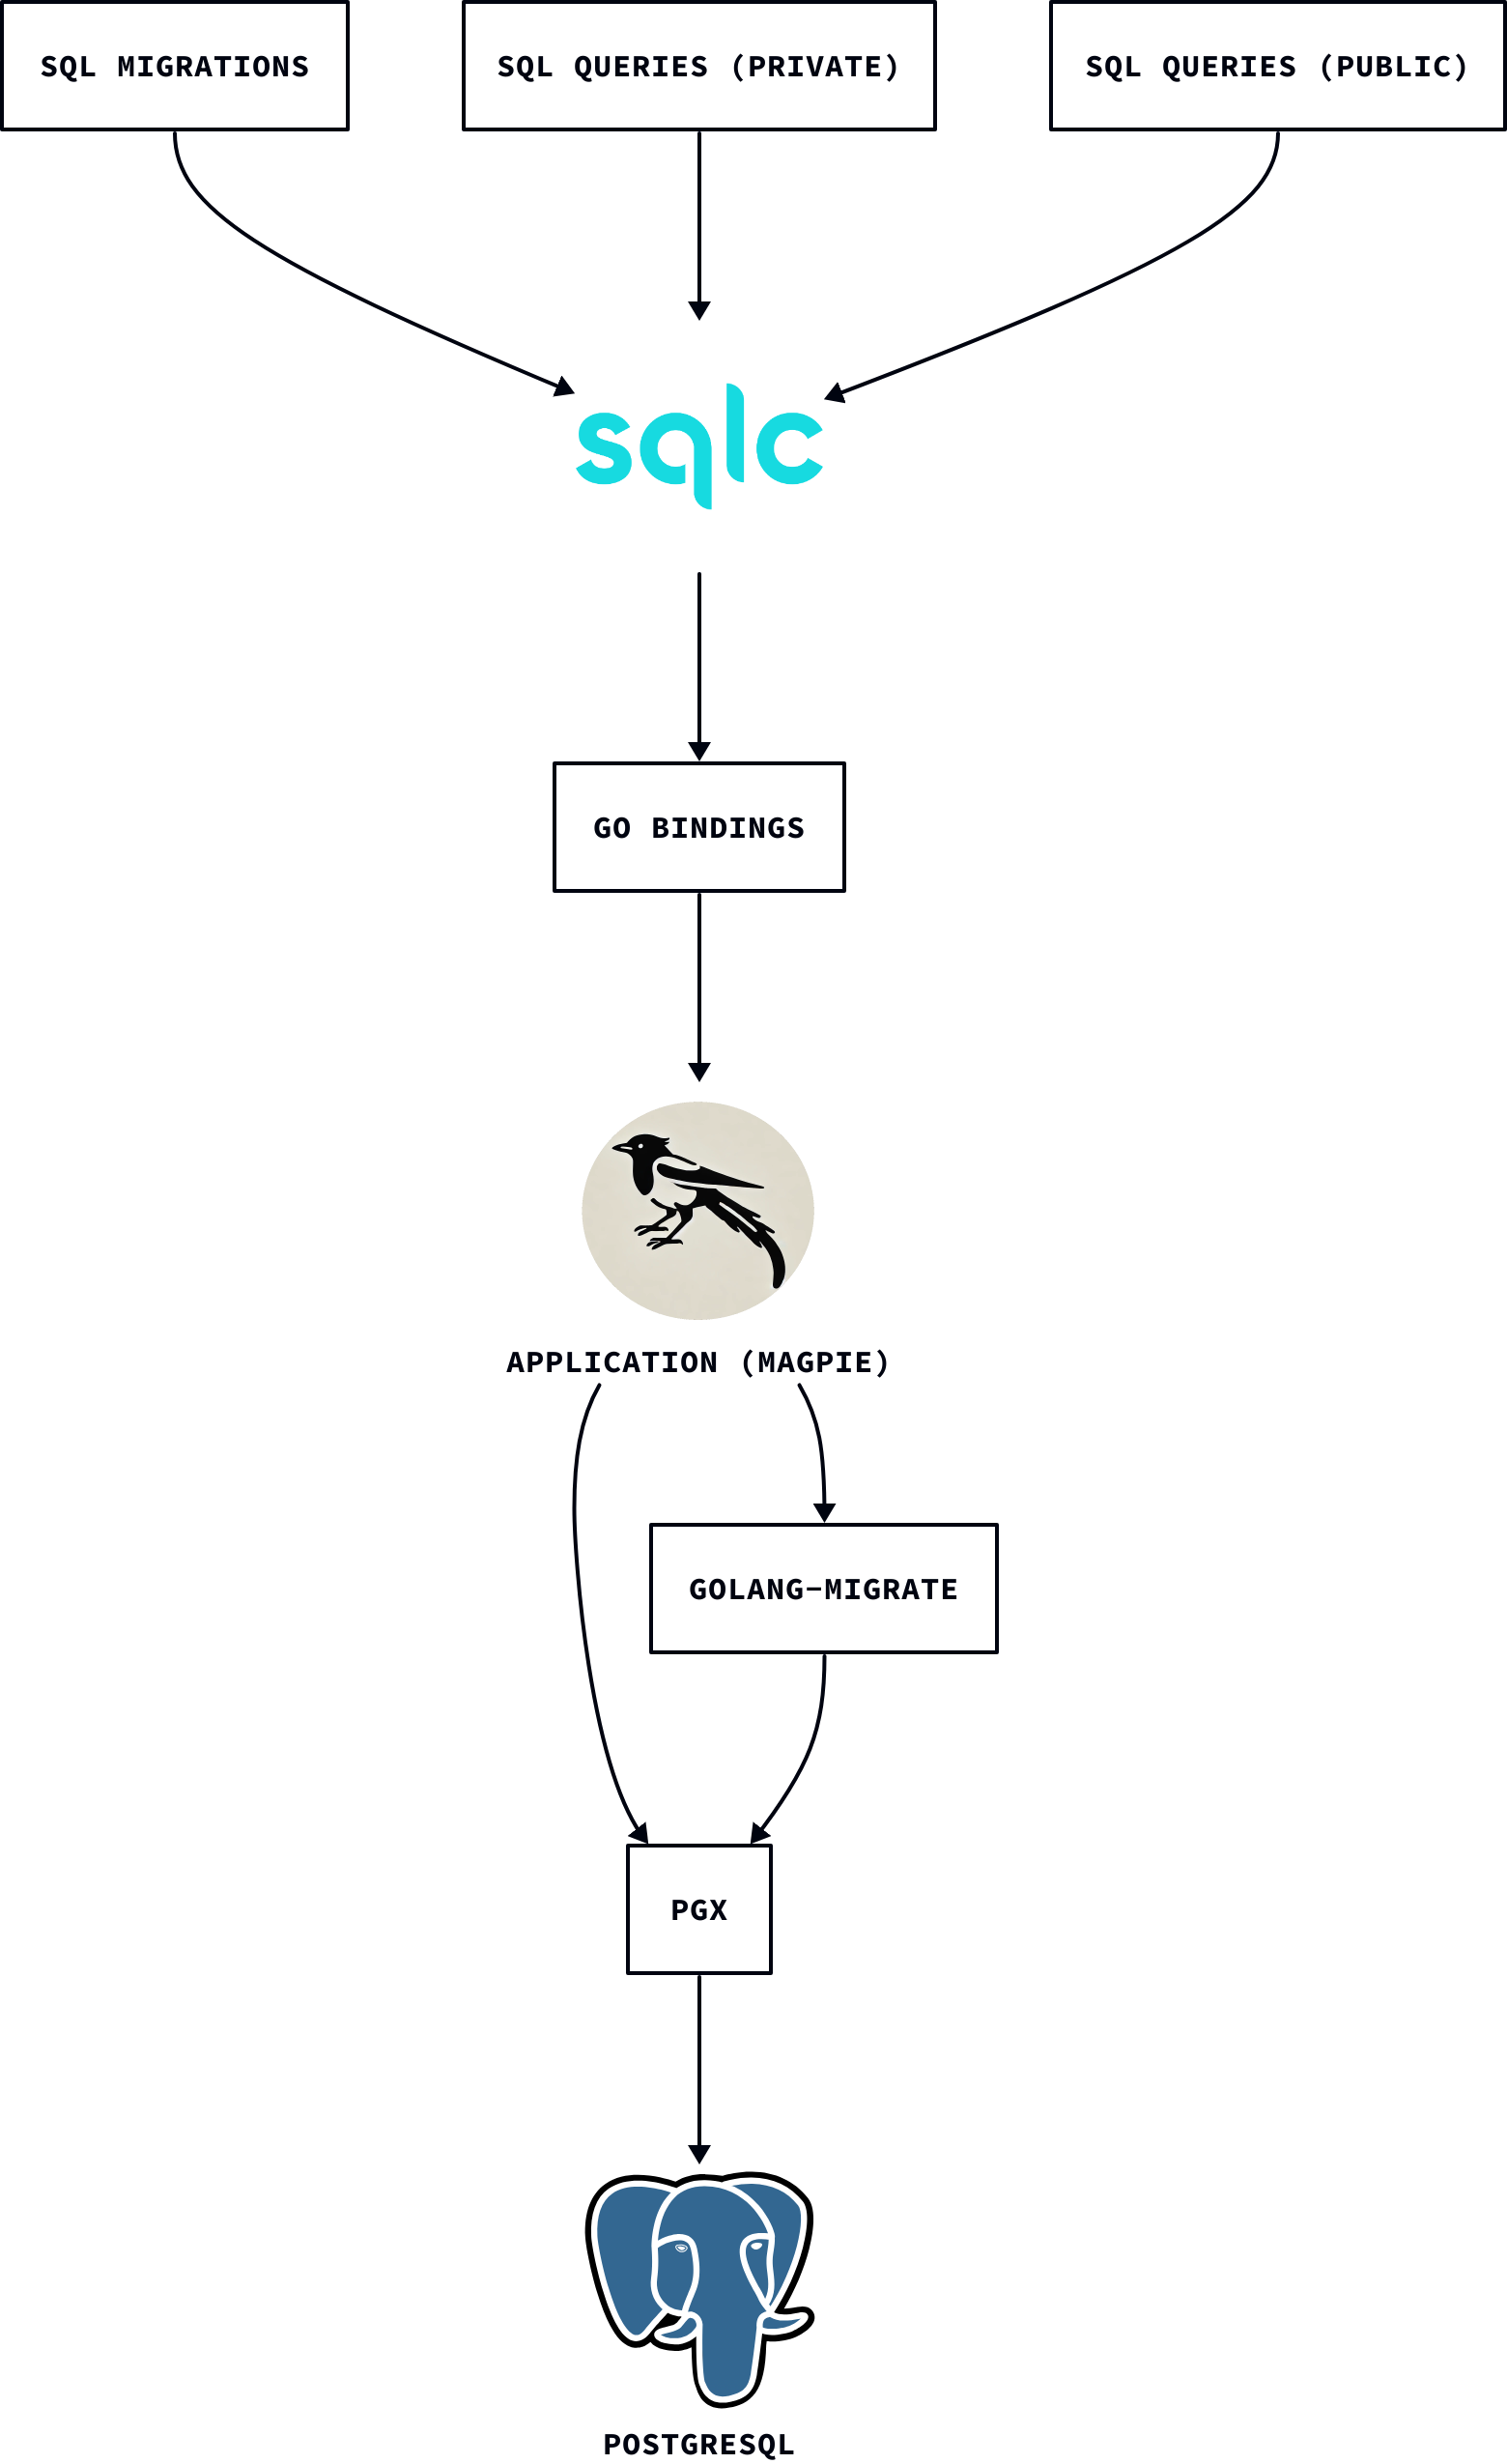
\includegraphics[width=0.8\textwidth]{../d2-diagrams/database-workflow/database_workflow.png}
  \caption{Database Workflow Diagram}
  \label{fig:database_workflow_diagram}
\end{figure}

\textbf{bcrypt}\\
To store the users credentials securely, \textbf{bcrypt} was chosen to hash them
before they are inserted into the database. The resulting hashes (see Figure
\ref{fig:bcrypt_hash}) can then be used to validate if the given password is
correct. In accordance with best practices, a work factor of 12 was used when
hashing passwords and a password limit of 72 bytes was implemented
(\cite{owasp_password_storage_cheatsheet}).

While the \textcite{owasp_password_storage_cheatsheet} recommends other, more
recent technologies over bcrypt, they also don't discourage its use in any way.
In the case of Magpie, bcrypt was chosen because the team had past experience
working with it. This was desirable as the registration and login functionality
was deemed to be one of the core features of the MVP. Choosing a technology that
the team did not have any experience with could have resulted in slower
development, bugs, or even security vulnerabilities as a result of improper
implementation.

Since the application was not intended to store highly valuable personal data
such as banking information, personal addresses or health care records it was
deemed acceptable to use a less recent technology in exchange for more rapid
development. Should this project ever evolve into a publicly available and
frequently used application, the use of bcrypt would of course need to be
reevaluated with a much bigger focus on real-world application security rather
than just development speed.

\begin{figure}[H]
  \centering{}
  
\includegraphics[width=0.8\textwidth]{./images/bcrypt_hash.png}
  \caption{Visualisation of a bcrypt hash}
  \label{fig:bcrypt_hash}
\end{figure}

\phantomsection\label{jwt}\textbf{JSON Web Token}\\
\textbf{JSON Web Tokens} were chosen for the authentication of user requests to
the APIs. JWTs are JSON objects that are encrypted using a private key on the
server and passed to the frontend when a login requests succeeds. The client is
then expected to pass the token to the backend as a form of authentication in
subsequent requests.

JSON Web Tokens are more than just a simple API token. They can store data about
the authenticated user in them, which can be very useful if the handling of the
requests needs a reference to the user id for example (see example JWT content
in Figure \ref{fig:jwt_example}). Since the tokens are generated on the backend
server using a private secret, JWTs can be checked for integrity during
decoding. Should the content not match up with the private secret of the backend
server, it can be assumed that the token has been tempered with. In this case,
the request would be discarded and an "Unauthorized" error message would be
returned instead.

This structure allows for the authentication system to be decoupled between
backend and frontend. Using JWTs eliminates the need for the backend to keep
track of active sessions, significantly reducing complexity. This and the
familiarity the team had with working with JWTs were ultimately chosen as the
authentication solution for Magpie.

JSON Web Tokens do however come with their own caveats. For example, if any
malicious actor stole such a token from a user, they could pretend to be that
user without the system noticing. JWTs do not have a built-in way to revoke
potentially stolen tokens, neither from the client nor from the server
(\cite{owasp_jwt_cheatsheet}).

Despite these caveats and some slowdowns during development, the team still
feels JWT-based authentication was the right choice for a project of Magpie's
scale.

\begin{figure}[htbp]
  \centering{}
  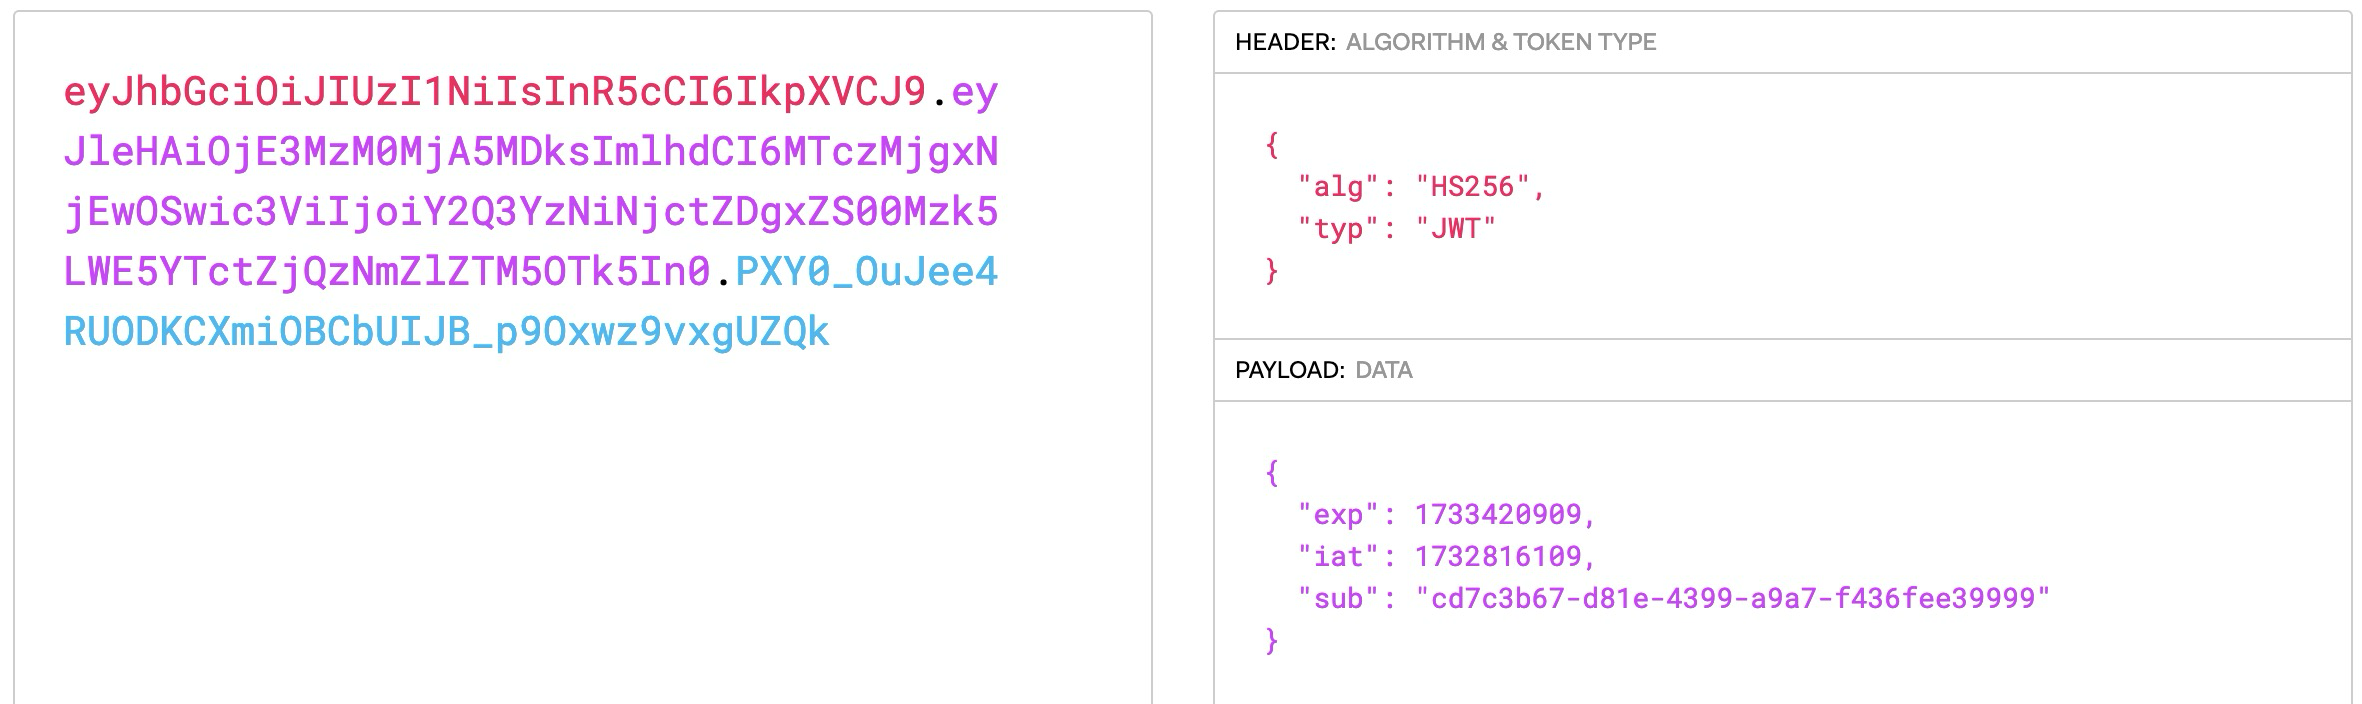
\includegraphics[width=\textwidth]{images/jwt.png}
  \caption{Example of a JWT used by Magpie for authenticaion}
  \label{fig:jwt_example}
\end{figure}

\subsubsection{Split Backend}
The backend was planned as a one server system, but the team wanted to harden
the system as a whole against potential attacks. This meant that some critical
functionality could not be included in the server that handles public requests.
As a result, the backend is comprised of two standalone REST-API servers. Both
of these servers access a shared database, allowing them to cooperate without
sharing functionality. The private backend is used to insert datasets into the
database, the public backend is used to retrieve that data from the database and
pass it to the frontend server.

This means that even if a malicious actor gained access to the public backend
server, they could not execute anything that would threaten the integrity of the
datasets stored in the database.

Right after the decision to split the backend was taken, a first implementation
using two separate codebases was created. This approach was functional, meaning
it was able to produce two distinct backends with different feature sets.

But it soon became obvious that this approach was not sustainable. While simply
splitting the backend into two codebases was a quick and easy solution, it would
almost certainly lead to significantly increased development times in the
future. The two backends have a fair amount of identical functionality and
differ just in the route handlers and the database queries. Leaving the
codebases separate would result in many changes being made twice -- once in the
private backend and once in the public backend.

After careful consideration and discussions with the team, the decision was made
to revert the change that split the backend. The desired result of two distinct
backends would have to be achieved in a different way.

To accomplish this, a feature of the Go programming language called
\textbf{build-tags} was utilised. Usage examples of this feature showcase it by
creating multiple binaries that have different feature sets, for instance
multiple different payment tiers for a single software. This was a great
solution for this problem. It allowed for certain files to be excluded during
compilation based on if they were needed for private or public functionality.
While the development of a program split by build-tags is more challenging
than developing a single binary, it is much more streamlined than keeping
functionality identical between two separate projects.

The build-tag system did not fix the problem of code duplication completely
however. Some tools in the Go ecosystem did not handle the exclusive split as
expected. Most notably, the Go language server that provides code completion and
other useful IDE features. It was possible to configure it to recognise files
with their accompanying build-tags, but there was no way to specify exclusivity.
This meant that two files in the same package could not have identical function
definitions even though they would never be included in the binary build process
simultaneously. It was possible to work around this restriction, which it lead
to some code duplication. But this was still a lot better than duplicating the
whole backend.

And while sqlc offers integration for the build-tag system (see the config file
in Listing \ref{listing:sqlc_config_file}), it did not offer to just split the
query part of the generated bindings. As a consequence, the generated code
handling the model bindings and the access to the database had to be generated
and included twice.

\subsubsection{Database Development}\label{database_development}
The requirements for the database of the MVP were simple: store points, store
users. To achieve this, three tables and one enum were added. The
\texttt{Points} table is used to store the actual data for Magpie. In the first
iteration (see Figure \ref{fig:database_init_schema}), this was only parking
spots detected by the machine learning stack.

The tables \texttt{Logins} and \texttt{User\_Details} are used to hold account
information. This design is a one-to-one relationship, which is usually
discouraged in database design. However, data from the \texttt{Login} table and
data from the \texttt{User\_Details} table are never queried at the same time
but only separately. While this design still violates database normalisation
principles, it makes querying the data more straightforward and was therefore
preferred in this time-constrained project.

Encoding the point type in an enum has benefits and drawbacks. Using an enum
enforces stricter data integrity, only a point with a type that is present in
the enum can be inserted into the database. By extension, this helps to
standardise the names of point types accross all layers of the application. On
the other hand, storing the point type in an enum makes the database a lot less
flexible. Adding a new dataset will almost certainly require changing the point
type in the database. This creates a barrier to quickly expanding the number of
different datasets in Magpie. Creating what is essentially a custom data type in
the database also led to issues with connecting the backend to the database. The
driver used for this purpose (\texttt{pgx}) expects custom data types to be
registered on the database connection instance. Figuring out how to do that
acted as a blocker for further backend development. It was still possible to add
new datasets, but the decision to store the point type in an enum should be
re-evaluated for future projects.

The \texttt{Schema\_Migrations} table seen in both the initial database schema
as well as in the final database schema is automatically created by
golang-migrate to track the current version of the database.

\begin{figure}[htbp]
  \centering{}
  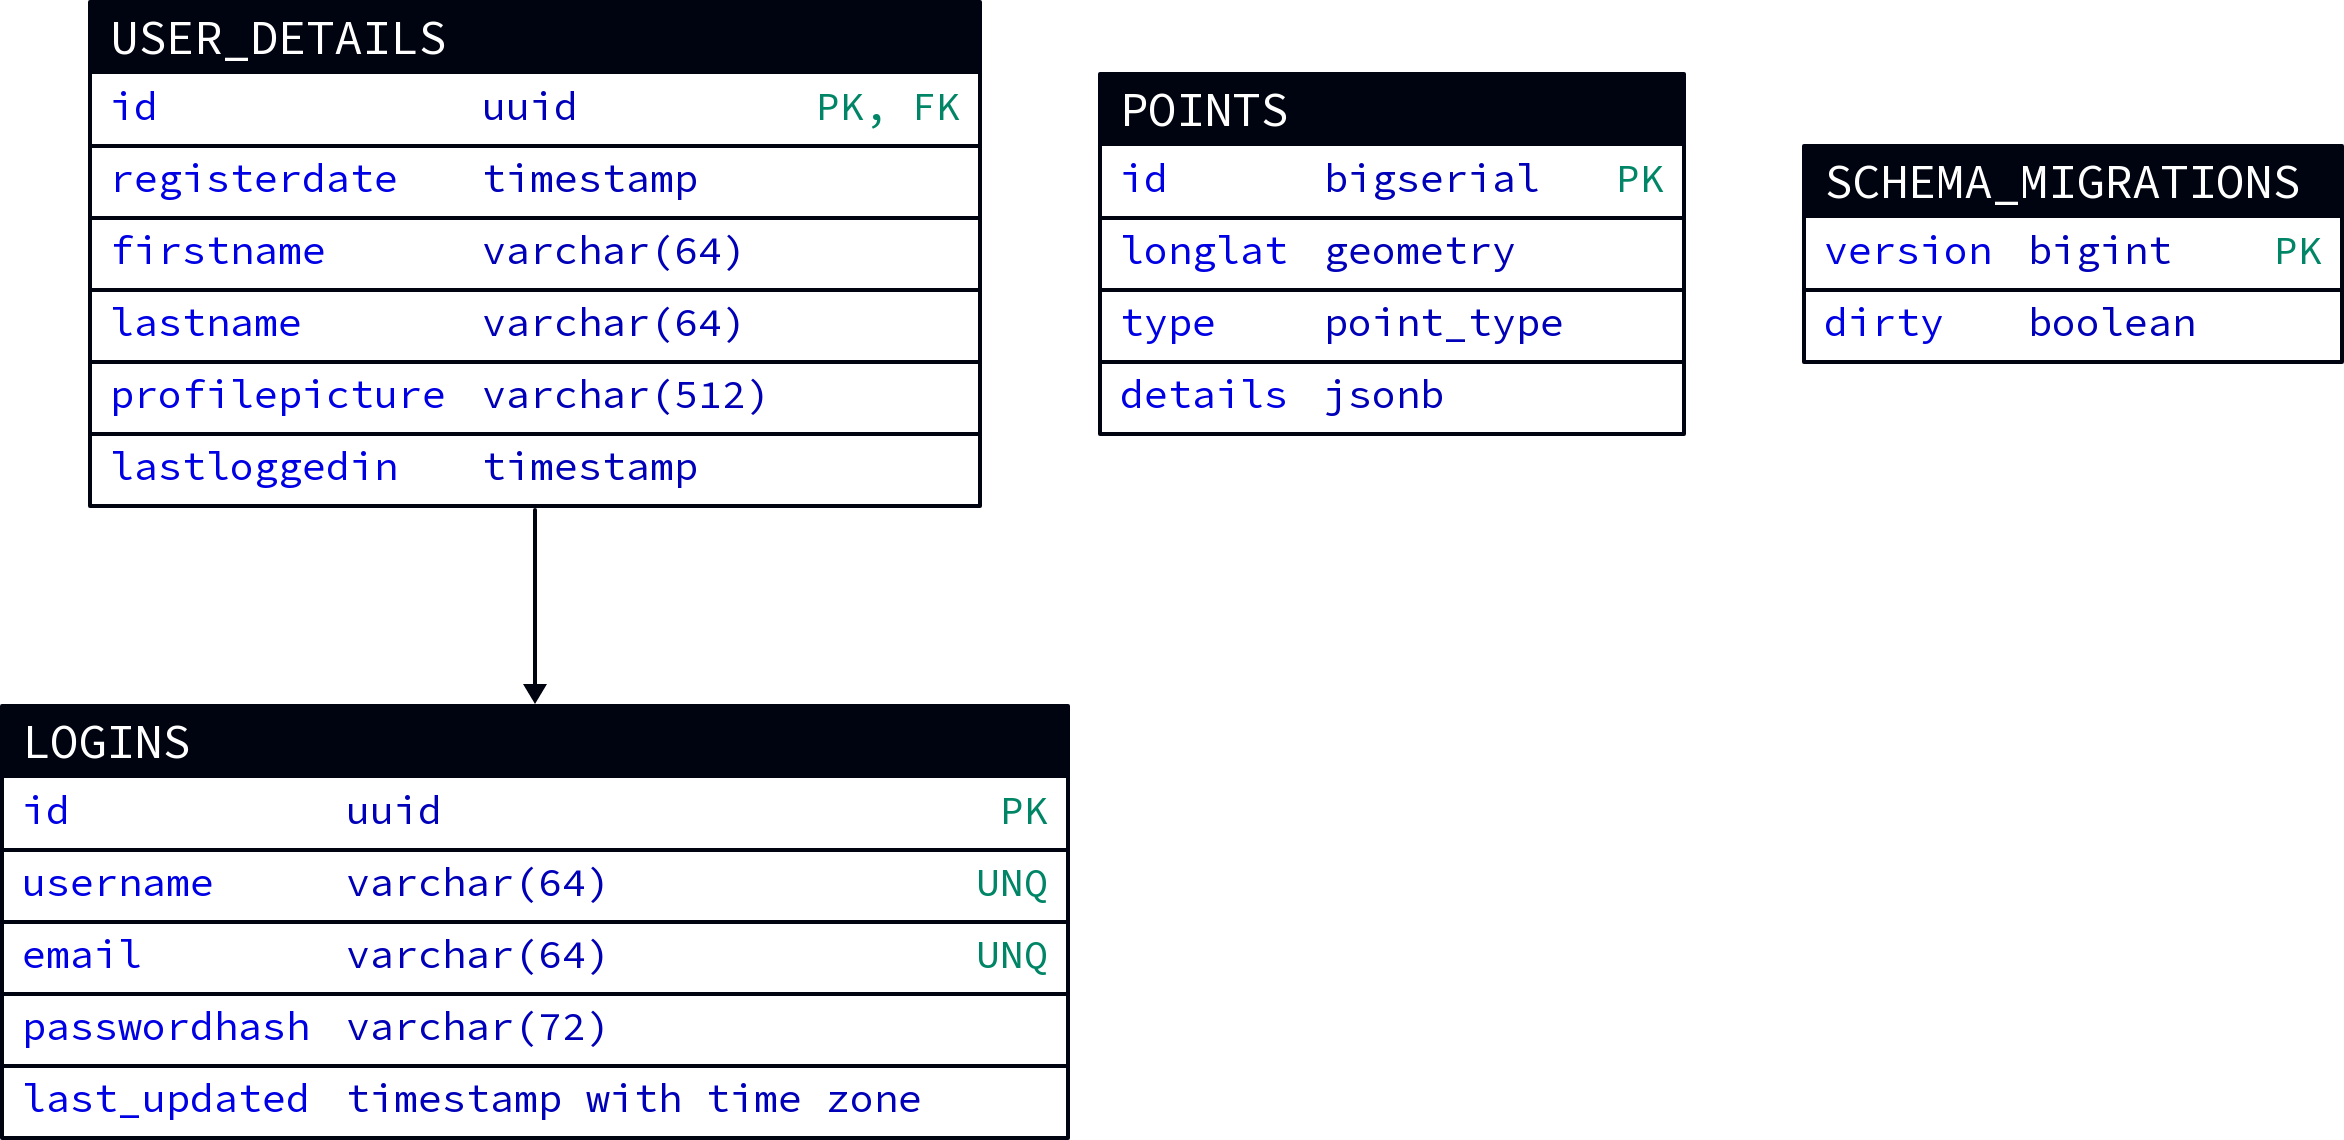
\includegraphics[width=\textwidth]{../d2-diagrams/database-init/database-init.png}
  \caption{Database Schema for the minimum viable Product}
  \label{fig:database_init_schema}
\end{figure}

During the course of the project, two significant changes were made to the
database. The first one was the addition of more point types to the
\texttt{Point\_Type} enum. To make it possible to seamlessly move between
database versions, migrations were designed to be reversible and (where
possible) prevent data loss.

Unfortunately, PostgreSQL only allows the addition of enum values but not the
deletion. Because of this, the down (reverse) migration for this change have to
use a workaround. First, a transaction is started, then the existing enum is
renamed and a new enum is created under the original name with the necessary
values already removed. Afterwards, the \texttt{Points} table is modified to use
the newly created enum. The old enum is then dropped and the transaction
committed.

To satisfy the goal to have as little data loss as possible when moving through
migrations, any point whose type is removed by a migration will have it added to
a special value in the \texttt{details} field. Should the migration ever be
re-applied, this field is then taken from the \texttt{details} object and
translated into the correct enum again. Since all points need to have a point
type, points whose type was removed will be given the type \texttt{unknown}. If
down migrations are executed past the point where the \texttt{unknown} type was
added, data loss is inevitable.

The second big change was the addition of the saved locations feature. This was
originally called 'History', which is why the database tables are still called
\texttt{Location\_History} and \texttt{History\_Amenity\_Counts}. At first, only
the former table was created, but as the feature evolved it became necessary to
store a place name (called \texttt{displayname} in the database) and counts of
amenities along side the saved location. This was also realised using migrations.

The \texttt{History\_Amenity\_Counts} table has a one-to-many relationship with
the \texttt{Location\_History} table, making it possible to include zero or more
amenities in the saved location. There can only be zero or one entries for each
point type per saved location. This is enforced by including both the point type
and the id of the saved location entry in the primary key constraint.

The final database schema is shown in Figure \ref{fig:database_final_schema}.

The team recognises that neither the database nor the queries can be considered
fully optimised. This was a concious choice, trading some performance for
quicker development time. Benchmarks of the point retrieval query performed by
the team showed that the database took less than 100ms to retrieve 58,192 rows
of points in a radius of 10 kilometres. The time it took to for the data to be
transmitted to and be parsed by the frontend was in excess of 1.4 seconds. While
there are performance bottlenecks in Magpie, the database's performance is
currently not considered one of them.

\begin{figure}[htbp]
  \centering{}
  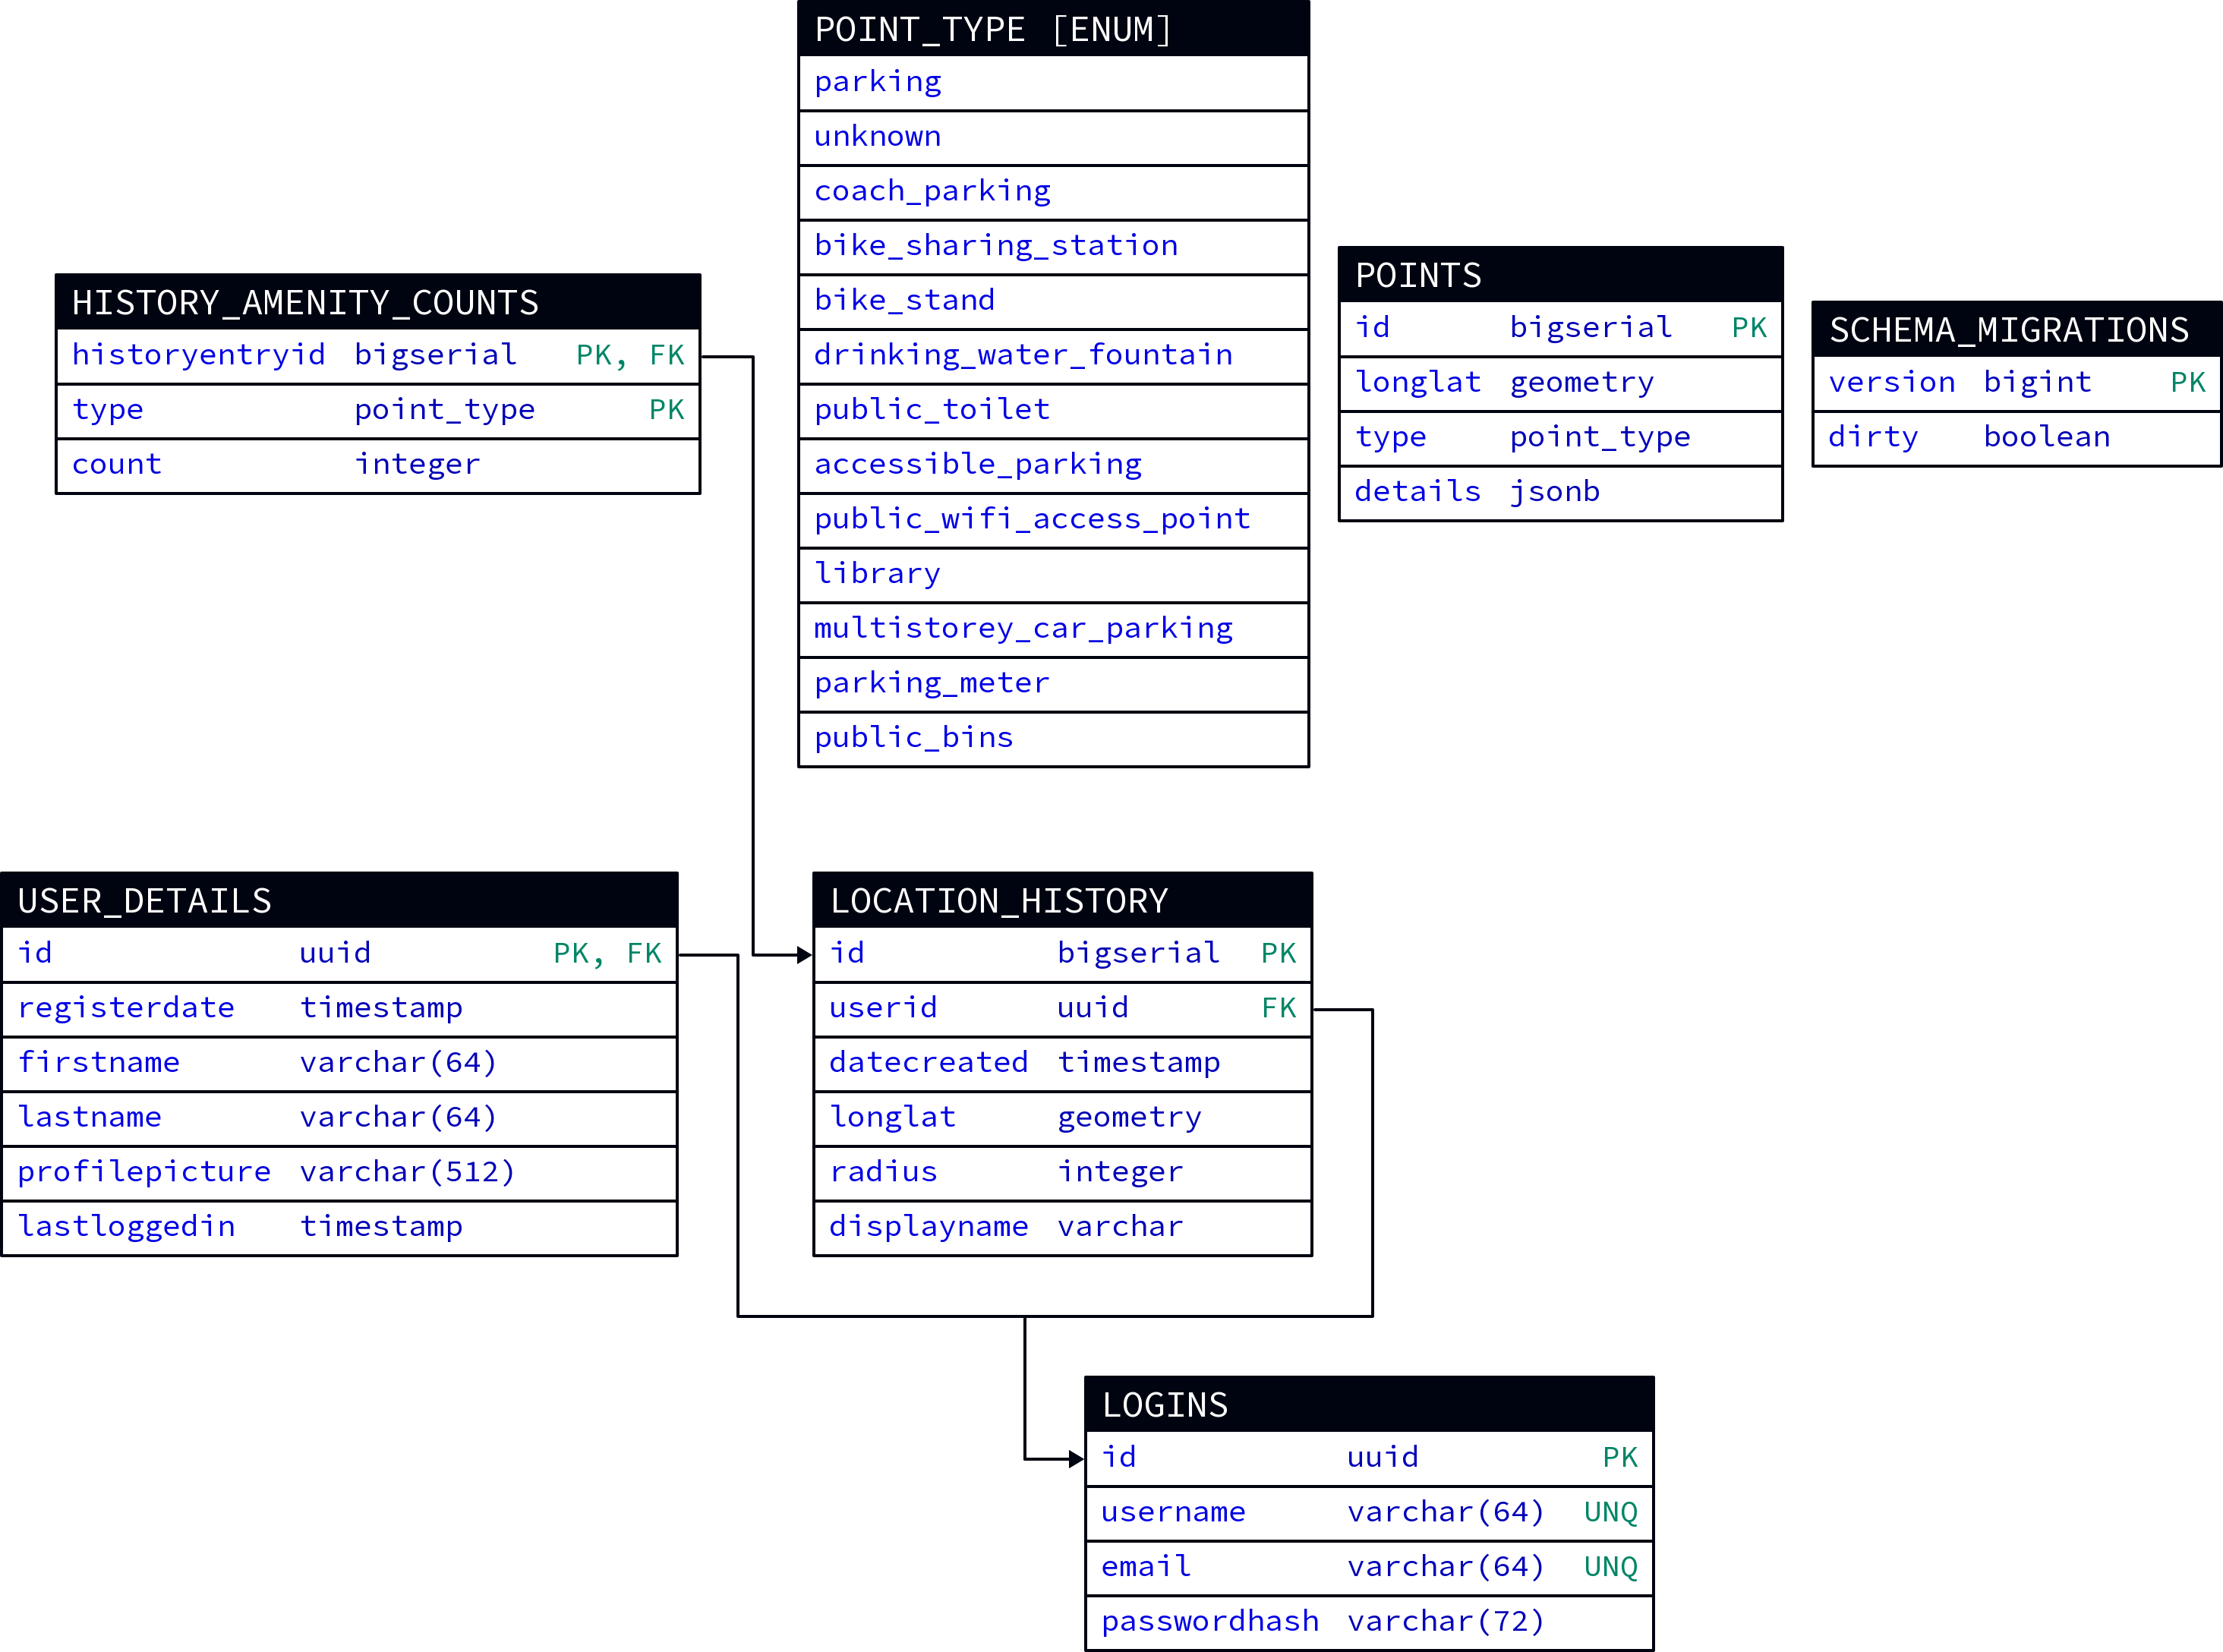
\includegraphics[width=\textwidth]{../d2-diagrams/database-final/database-final.png}
  \caption{Final Database Schema}
  \label{fig:database_final_schema}
\end{figure}

\subsubsection{Routing}
Routing the frontend's requests to the appropriate handlers was done using the
\textbf{net/http} package, which is included in the Go standard library. The Go
ecosystem provides a number of alternative solutions such as Gin, Gorilla or
Fibre, which are mature and well documented frameworks for creating APIs. They
provide many useful features, which the team acknowledged during their
evaluation, but -- in the team's opinion -- they can also easily add a lot of
complexity. Since the team was lacking in recent Go knowledge and didn't want to
unnecessarily overcomplicate the project, it was decided to go with the built-in
solution instead.

To realise the API functionality, the http server function provided by the
net/http library is configured with a \texttt{http.ServeMux} object. This is
where the server will send all incoming requests. These are then passed to
nested routers based on prefix routing. For example, a request for the route
\texttt{/v1/public/auth/User/login} would follow this path: HTTP Server
$\rightarrow$ Public Router $\rightarrow$ Public Auth Router $\rightarrow$ Auth
handler. A full overview of the routing in the backend can be found in Figure
\ref{fig:backend_routing}.

All requests are also routed through a stack of middlewares. Some middlewares
are active on all requests (Logging, CORS) and some are configured based on
route (Authorisation), see Section \ref{backend_middlewares}
(\nameref{backend_middlewares}).

\begin{figure}[htbp]
  \centering{}
  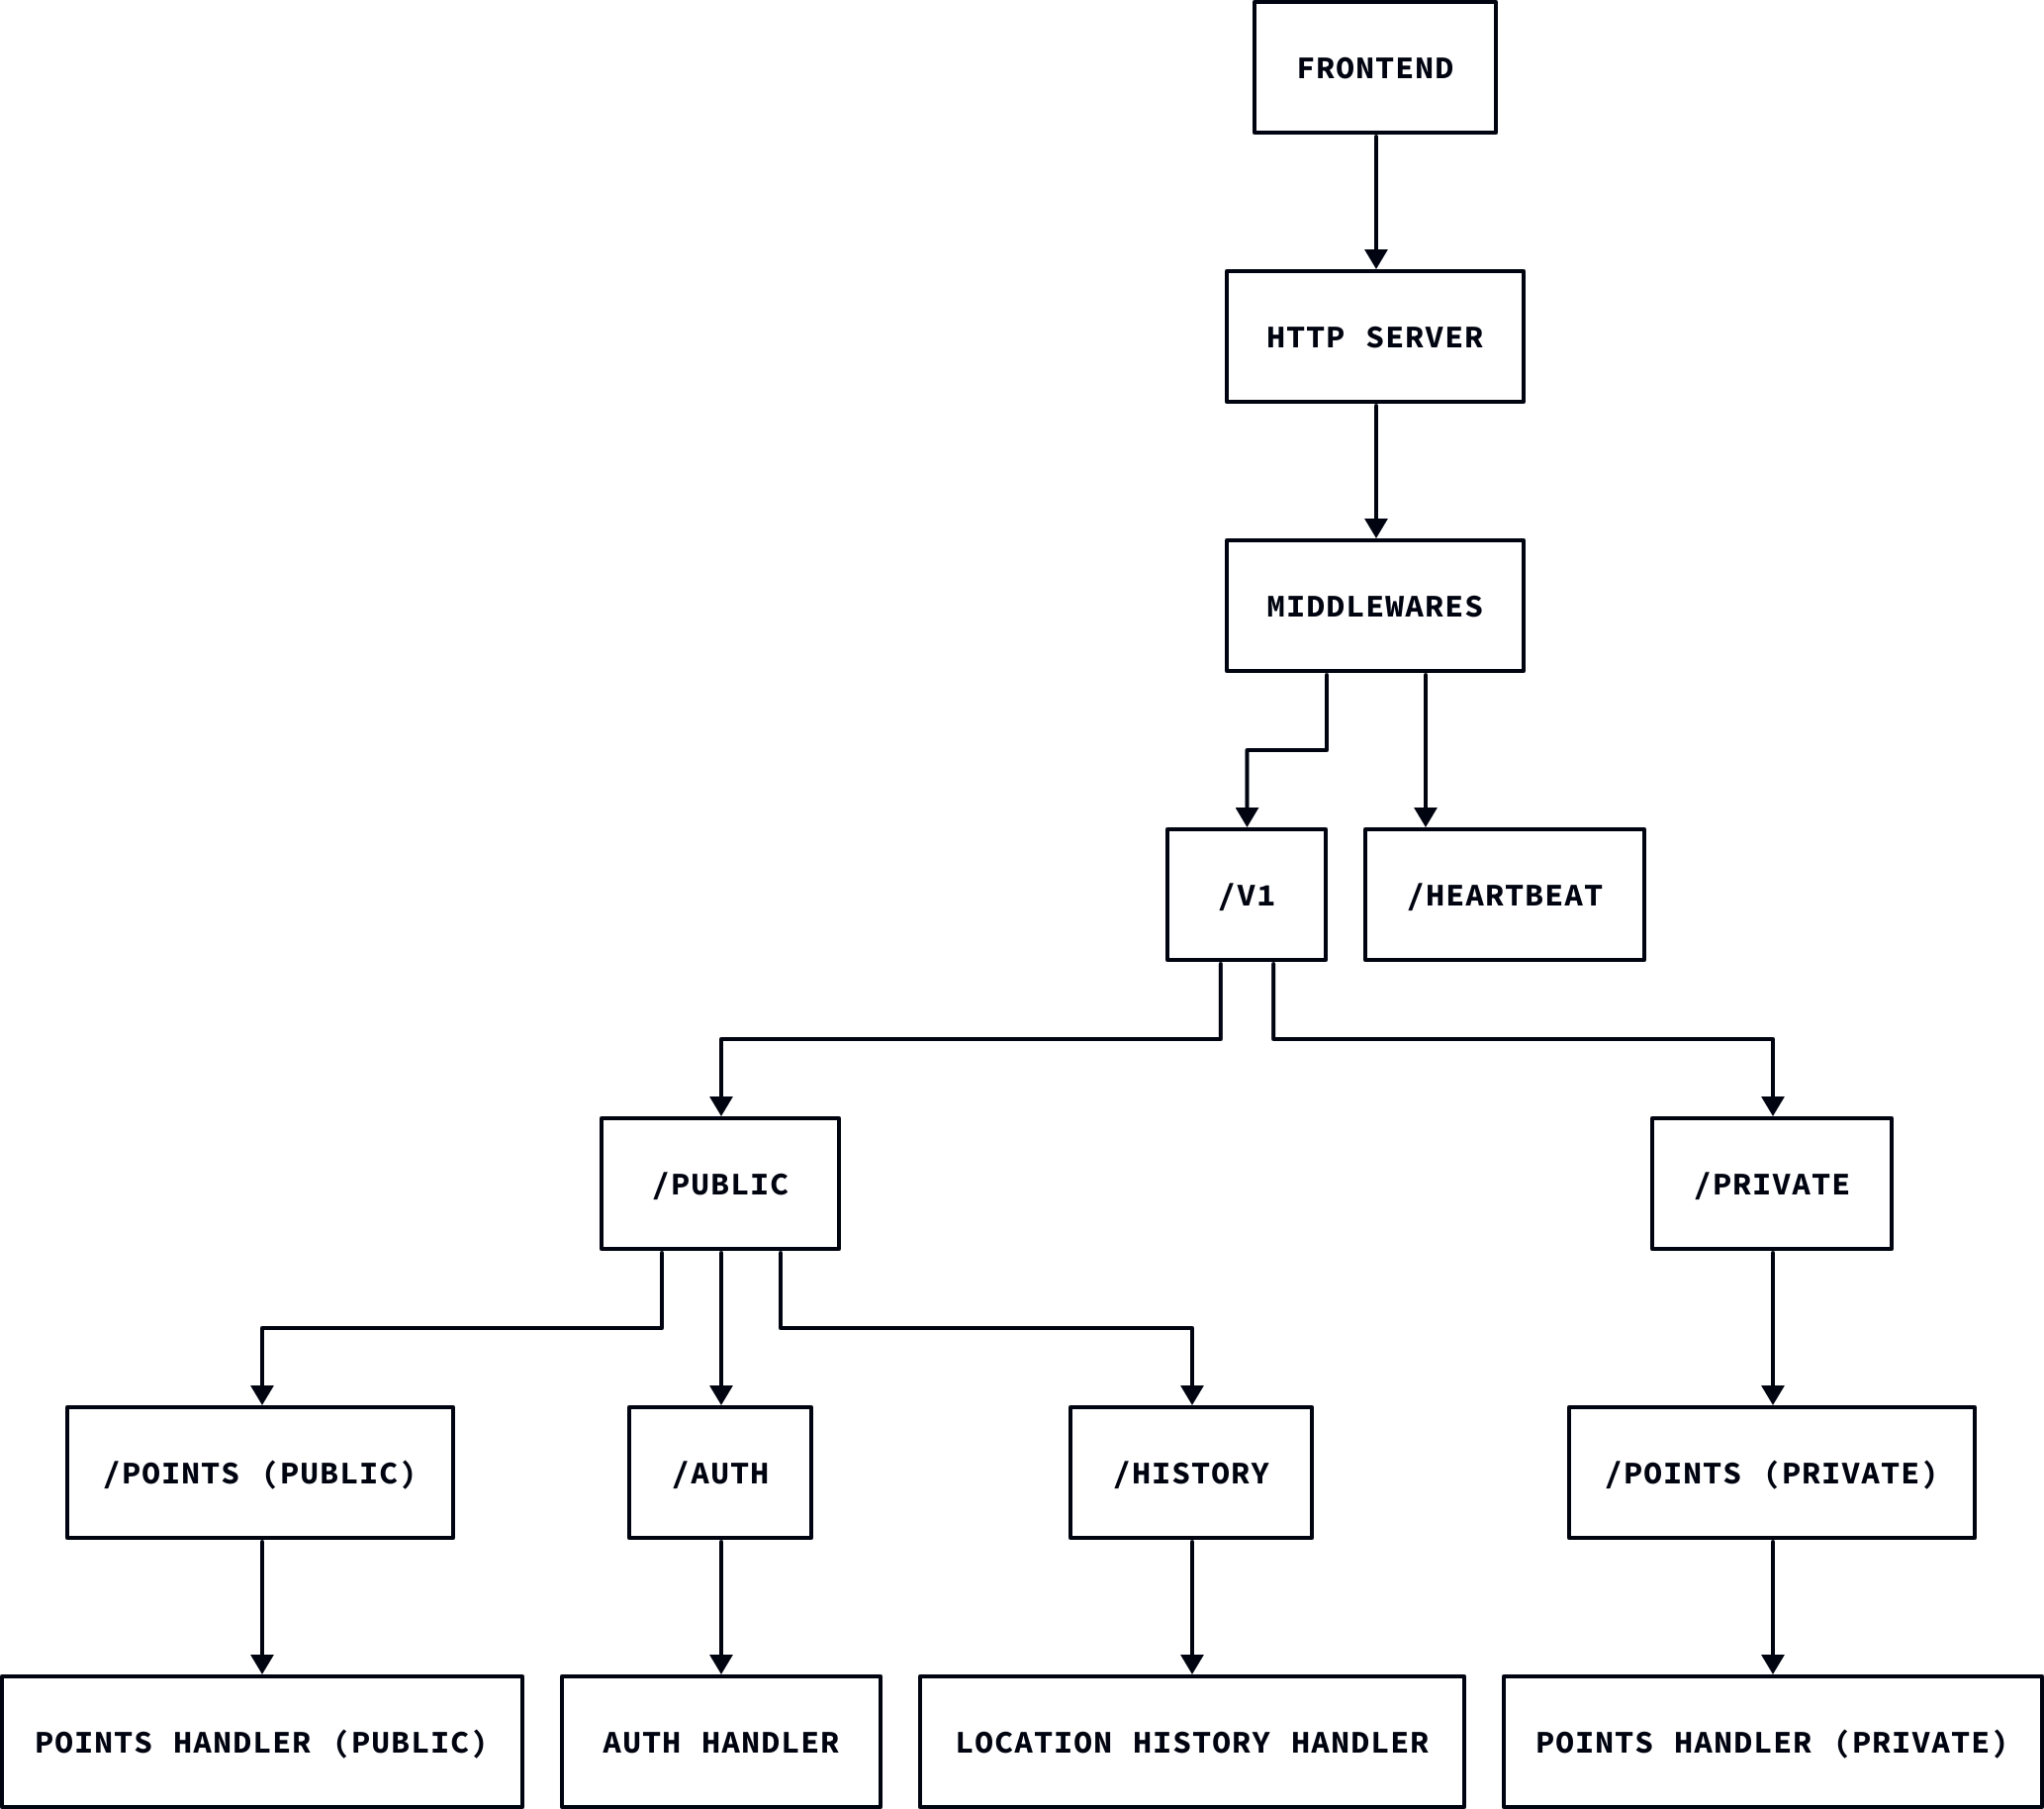
\includegraphics[width=\textwidth]{../d2-diagrams/backend-routing/backend-routing.png}
  \caption{Routing in the Backend: from Request to Handler}
  \label{fig:backend_routing}
\end{figure}

\begin{listing}[htbp]
  \begin{minted}[fontsize=\footnotesize]{go}
func init() {
  AddRoute(route{"/public/", public()})
}

func public() *http.ServeMux {
  router := http.NewServeMux()
  router.Handle("/points/", http.StripPrefix("/points", pointsPublic()))
  router.Handle("/auth/", http.StripPrefix("/auth", auth()))
  router.Handle("/history/", http.StripPrefix("/history", locationHistory()))
  return router
}

func pointsPublic() *http.ServeMux {
  router := http.NewServeMux()
  handler := &handlers.PointsHandler{}

  // Authenticated access
  router.Handle("GET /inRadius", Authenticated(http.HandlerFunc(handler.HandleGetByRadius)))
  router.Handle("GET /{id}", Authenticated(http.HandlerFunc(handler.HandleGetPointDetails)))

  return router
}

func auth() *http.ServeMux {
  router := http.NewServeMux()
  handler := &handlers.AuthHandler{}

  // Public access
  router.Handle("POST /User/login", Public(http.HandlerFunc(handler.HandleLogin)))
  router.Handle("POST /User/", Public(http.HandlerFunc(handler.HandlePost)))

  // Protected access
  router.Handle("GET /User/{id}", Protected(http.HandlerFunc(handler.HandleGet)))
  router.Handle("PUT /User/{id}", Protected(http.HandlerFunc(handler.HandlePut)))
  router.Handle("DELETE /User/{id}", Protected(http.HandlerFunc(handler.HandleDelete)))

  return router
}

func locationHistory() *http.ServeMux {
  router := http.NewServeMux()
  handler := &handlers.LocationHistoryHandler{}

  // Protected access
  router.Handle("GET /{id}", Protected(http.HandlerFunc(handler.HandleGet)))
  router.Handle("DELETE /{id}", Protected(http.HandlerFunc(handler.HandleDelete)))
  router.Handle("POST /{id}", Protected(http.HandlerFunc(handler.HandlePost)))

  return router
}
  \end{minted}
  \caption{An example of how routing is configured in the backend}
  \label{listing:routing_example}
\end{listing}

\subsubsection{APIs}
All API routes that the backends expose are listed below. This information was
available to the frontend and data stack developers throughout the project in
the form of a collection of markdown files in the repository. This clearly
communicated the capabilities of the API routes, making it easier to develop the
application parts that interfaced with them. Providing strong documentation also
eliminated a lot of ambiguity, resulting in more concise and effient
communication between the different areas of responsibility.

For a detailed explanation of the route access restriction modes, see Section
\textbf{\nameref{middleware_route_authorisation}} on page
\pageref{middleware_route_authorisation}.

\newpage{}

\textbf{Public API}\\
The public API is used to retrieve relevant data for display in the frontend and
for authentication of the user.

\begin{itemize}
  \item{
    \textbf{Point Routes}
    \begin{itemize}
      \item { \textbf{Name:} Point Details\\
          \textbf{Method + Route:} \texttt{GET /v1/public/points/\{id\}}\\
          \textbf{Description:} Provides additional details about a point. The
          structure and content of the details is different for every point
          type. The details are derived from the input dataset and added to each
          point on ingress.\\
          \textbf{Access:} Authenticated\\
          \textbf{Parameters:} Point UUID (path parameter)\\
          \textbf{Returns:} JSON Object containing details about the point\\
        }
      \item { \textbf{Name:} Points in Radius\\
          \textbf{Method + Route:}\\\texttt{GET
          /v1/public/points/inRadius?long=\{\}\&lat=\{\}\&radius=\{\}\&types=\{\}}\\
          \textbf{Description:} Retrieves all points in a circle. The circle is
          defined by its center coordinates and a radius in meters. The
          \texttt{types} parameter is optional. If a comma separated list of
          point types is provided, the returned data will be filtered to only
          contain points with the given types.\\
          \textbf{Access:} Authenticated\\
          \textbf{Parameters:} Longitude, Latitude, radius, types (all query
          parameters)\\
          \textbf{Returns:} JSON object containing a list of points inside the
          given radius, filtered by the given point types\\
        }
    \end{itemize}
  }
  \item{
    \textbf{Saved Location Routes}
    \begin{itemize}
      \item {
        \textbf{Name:} Retrieve saved locations\\
        \textbf{Method + Route:} \texttt{GET /v1/public/history/\{id\}}\\
        \textbf{Description:} Retrieves all saved locations for the account
        specified by the user id. In previous versions, this route included
        pagination functionality, but due to the requirements of a frontend
        library, the backend now returns all saved locations.\\
        \textbf{Access:} Restricted\\
        \textbf{Parameters:} User UUID (path parameter)\\
        \textbf{Returns:} JSON object containing a list of all saved locations
        (including location, radius, number of amenities) for the specified
        user.\\
      }
      \item {
        \textbf{Name:} Delete saved locations\\
        \textbf{Method + Route:} \texttt{DELETE /v1/public/history/\{id\}}\\
        \textbf{Description:} This route allows the user to delete one or more
        of their saved locations. The route only deletes saved locations that
        are associated with the currently active account. Should this route
        receive ids of saved locations that are associated with another account
        or that don't exist, it simply ignores them.\\
        \textbf{Access:} Restricted\\
        \textbf{Parameters:} User UUID (path parameter), List of saved location
        ids (request body)\\
        \textbf{Returns:} Status 202 if no errors occurred during deletion.\\
      }
      \newpage{}
      \item {
        \textbf{Name:} Save location\\
        \textbf{Method + Route:} \texttt{POST /v1/public/history/\{id\}}\\
        \textbf{Description:} Creates a new saved location for the currently
        active user.\\
        \textbf{Access:} Restricted\\
        \textbf{Parameters:} User UUID (path parameter), JSON Object describing
        the saved location (request body)\\
        \textbf{Returns:} Status 201 if the location was saved successfully.\\
      }
    \end{itemize}
  }
  \item{
    \textbf{Authentication Routes}
    \begin{itemize}
      \item {
        \textbf{Name:} Create new account\\
        \textbf{Method + Route:} \texttt{POST /v1/public/auth/User/}\\
        \textbf{Description:} Allows users to create a new account. Both the
        backend and database will perform uniqueness checks on the given email
        and username. First name and last name are optional. The given password
        will be hashed before being stored in the database.\\
        \textbf{Access:} Public\\
        \textbf{Parameters:} JSON object containing all information for the new
        account (request body)\\
        \textbf{Returns:} The UUID of the new account and status 201 if the
        creation was successful.\\
      }
      \item {
        \textbf{Name:} Login\\
        \textbf{Method + Route:} \texttt{POST /v1/public/auth/User/login}\\
        \textbf{Description:} Allows users to retrieve an access token, given
        valid credentials.\\
        \textbf{Access:} Public\\
        \textbf{Parameters:} JSON object containing a password and a username or
        email.\\
        \textbf{Returns:} A JWT bearer token and the user UUID if the login was
        successful.\\
      }
      \item {
        \textbf{Name:} Get user details\\
        \textbf{Method + Route:} \texttt{GET /v1/public/auth/User/\{id\}}\\
        \textbf{Description:} Retrieves the user details for the current user.
        This includes the users first name, last name, date of registration,
        date of last login as well as a link to a profile picture. Requests for
        the details of other users are denied.\\
        \textbf{Access:} Restricted\\
        \textbf{Parameters:} User UUID (path parameter)\\
        \textbf{Returns:} JSON object containing additional details about the
        user.\\
      }
      \item {
        \textbf{Name:} Update user details\\
        \textbf{Method + Route:} \texttt{PUT /v1/public/auth/User/\{id\}}\\
        \textbf{Description:} Allows the user to update their own user details.
        With the exception of a new password, all parameters must be passed to
        this route, even if they aren't changed. New usernames and emails are
        checked for uniqueness by the backend and database. Keeping the same
        username or email does not violate the uniqueness constraint.\\
        \textbf{Access:} Restricted\\
        \textbf{Parameters:} JSON object specifying username, email, [password],
        first name, last name and profile picture link.\\
        \textbf{Returns:} Status 202 if the data was successfully updated.\\
      }
      \item {
        \textbf{Name:} Delete account\\
        \textbf{Method + Route:} \texttt{DELETE /v1/public/auth/User/\{id\}}\\
        \textbf{Description:} Allows the user to delete their account. This also
        deletes all associated data like user details and saved locations. There
        is currently no way to undo this action.\\
        \textbf{Access:} Restricted\\
        \textbf{Parameters:} User UUID (path parameter)\\
        \textbf{Returns:} Status 202 if the request was accepted.\\
      }
    \end{itemize}
  }
  \item{
    \textbf{Status Routes}
    \begin{itemize}
      \item {
        \textbf{Name:} Heartbeat\\
        \textbf{Method + Route:} \texttt{GET /heartbeat}\\
        \textbf{Description:} This route is used by the automated deployment to
        check if the public backend is up and ready to receive connections. This
        helps alleviate issues with the starting order of services on a
        Kubernetes cluster.\\
        \textbf{Access:} Public\\
        \textbf{Parameters:} None\\
        \textbf{Returns:} \texttt{true} if the service is ready to receive
        connections.\\
    }
    \end{itemize}
  }

\end{itemize}

\textbf{Private API}\\
The private API is used by the machine learning and data stack to insert new
datasets into the database. Currently, all private API routes have public access
rights, as the private backend as a whole is guaranteed restricted access by the
CoreDNS routing of the Kubernetes cluster. This allows the data stack to skip
the authentication step, decreasing development overhead while maintaining high
application security.

\begin{itemize}
  \item {
    \textbf{Point Routes}
    \begin{itemize}
      \item {
        \textbf{Name:} Create new point\\
        \textbf{Method + Route:} \texttt{POST /v1/private/points}\\
        \textbf{Description:} Allows the data stack to create a new point in the
        database. Since the point details vary from point type to point type,
        they are stored in the database in the form of a JSON object. This also
        allows for less restrictions to the type of data that can be added here,
        making Magpie more flexible in development.\\
        \textbf{Access:} Public\\
        \textbf{Parameters:} JSON object containing the location of the point,
        the point type and a nested JSON object containing all the point
        details.\\
        \textbf{Returns:} The integer id of the newly created point.\\
      }
      \item {
        \textbf{Name:} Update point\\
        \textbf{Method + Route:} \texttt{PUT /v1/private/points/\{id\}}\\
        \textbf{Description:} This route allows the data stack to update a point
        that is already stored in the database. This is not currently used in
        Magpie, but it will be useful in the future as datasets will become
        outdated over time.\\
        \textbf{Access:} Public\\
        \textbf{Parameters:} Point id (path parameter), JSON object containing
        the points new data\\
        \textbf{Returns:} The point id and Status 202 if the update was
        successful.\\
      }
      \item {
        \textbf{Name:} Delete point\\
        \textbf{Method + Route:} \texttt{DELETE /v1/private/points/\{id\}}\\
        \textbf{Description:} Using this route, the data stack can delete a
        specific point from the database. This is currently not used in Magpie,
        but removing stale and outdated data will become necessary as time goes
        by.\\
        \textbf{Access:} Public\\
        \textbf{Parameters:} Point id (path parameter)\\
        \textbf{Returns:} Status 202 if the request was accepted.\\
      }
    \end{itemize}
  }
  \item{
    \textbf{Status Routes}
    \begin{itemize}
      \item {
        \textbf{Name:} Heartbeat\\
        \textbf{Method + Route:} \texttt{GET /heartbeat}\\
        \textbf{Description:} This route is used by the automated deployment to
        check if the public backend is up and ready to receive connections. This
        helps alleviate issues with the starting order of services on a
        Kubernetes cluster.\\
        \textbf{Access:} Public\\
        \textbf{Parameters:} None\\
        \textbf{Returns:} \texttt{true} if the service is ready to receive connections.\\
      }
    \end{itemize}
  }
\end{itemize}

\subsubsection{Middlewares}\label{backend_middlewares}
\phantomsection\label{middleware_route_authorisation}\textbf{Authorisation}\\
The backend implements three middlewares that allow for route-based
authorisation. Using this, some routes can be publicly accessible while others
are only available to authenticated users in general or specific users only.
This is accomplished by wrapping the handler function in the appropriate
middleware when configuring the routing, see Listing
\ref{listing:routing_example}.

The \textit{public access middleware} simply forwards the request to the
handler. This is used for routes that all users need access to, such as logging
in or account creation. The \textit{authenticated access middleware} extracts
the JWT from the request and checks it for validity. Only if the JWT is valid is
the request passed to the handler, if not, an error is returned.

The \textit{protected access middleware} only allows requests to user specific
resources that are made by that exact user. All routes with protected access are
also checked by the authenticated access middleware. The user id is then
extracted from the proven valid JWT. Comparing the extracted id with the user id
given in as a path parameter, it can be determined if the user making the
request is actually the owner of the resource. In that case, the request is
forwarded to the handler function. If the ids do not match, the request returns
an error.

\phantomsection\label{middleware_logging}\textbf{Logging}\\
The backend uses logs for monitoring purposes. The servers output informative
messages, warnings and errors. The latter two are essential for figuring out any
configuration issues with the server and are vital for debugging purposes. In
addition, every request that is handled by the backend is logged including its
status, route and precise execution time. This can be used to pinpoint requests
that are failing with regularity or take significant time to complete. An
example of the logs produced by the public backend server can be found in Figure
\ref{fig:backend_logging}.

\begin{figure}[htbp]
  \centering{}
  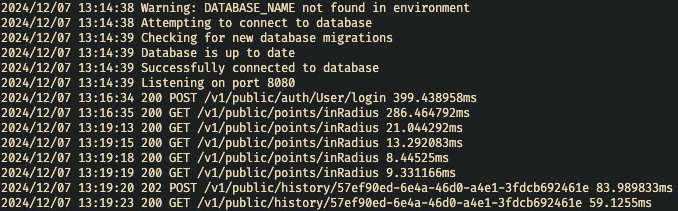
\includegraphics[width=0.7\textwidth]{images/backend_logging.png}
  \caption{Example of logs produced by the public backend server}
  \label{fig:backend_logging}
\end{figure}

\newpage{}

\phantomsection\label{middleware_cors}\textbf{Cross-origin Resource Sharing (CORS)}\\
Since the frontend and the backend are not hosted at the same origin, it is
necessary for the backend to enable cross-origin resource sharing. If this is
not done, the user's browser will block any requests made to the backend. There
was no need for custom CORS headers, so in the interest of simplicity an
existing library (\textbf{Go CORS handler}) was chosen for this purpose.

\subsubsection{Data Validation}
Data that enters Magpie is validated on ingress. At the most basic level, there
are checks for the presence of required parameters. But the data is also checked
for logical errors, such as coordinates having a longitude greater than 180/less
than \-180 degrees or a latitude greater than 90/less than \-90 degrees.

These checks are implemented in the data types that the incoming data is decoded
into called \textbf{Data Transfer Objects (DTOs)}. Since Magpie uses JSON
objects to transmit data, the decoding is handled by the built-in
\texttt{encoding/json} library. Should any parameter not match up with the
expected struct, the decoding fails. This is the first line of defence. In
addition, all DTOs implement a \texttt{Validate} function, that can be used to
specify any additional requirements for the incoming data. It is called
automatically once the decoding process has finished. An example of a DTO
definition can be seen in Listing \ref{listing:dto_example}.

While these checks cannot guarantee that the inserted data is actually correct,
they do improve data integrity. During development, the sanity checks have
proven to be instrumental in catching errors early when implementing a new
function that sends data to the API.

\newpage{}

\begin{listing}[htbp]
  \centering{}
  \begin{minipage}{0.75\textwidth}
  \begin{minted}{go}
type CreateUserDto struct {
  Username       string      `json:"username"`
  Email          string      `json:"email"`
  Password       string      `json:"password"`
  FirstName      string      `json:"firstname"`
  LastName       string      `json:"lastname"`
  ProfilePicture pgtype.Text `json:"profilepicture"`
}

func (self *CreateUserDto) Decode(r io.Reader) error {
  err := json.NewDecoder(r).Decode(&self)
  if err != nil {
    return customErrors.Payload.InvalidPayloadUserError
  }
  return self.Validate()
}

func (self *CreateUserDto) Validate() error {
  if len(self.Username) == 0 {
    err := customErrors.Parameter.
            RequiredParameterMissingError.
            WithCause(fmt.Errorf("Username is required"))
    return err
  }

  if len(self.Email) == 0 {
    err := customErrors.Parameter.
            RequiredParameterMissingError.
            WithCause(fmt.Errorf("Email is required"))
    return err
  }

  if len(self.Password) == 0 {
    err := customErrors.Parameter.
            RequiredParameterMissingError.
            WithCause(fmt.Errorf("Password is required"))
    return err
  }

  if len(self.Password) > 72 {
    err := customErrors.Payload.PasswordTooLongError
    return err
  }
  return nil
}
  \end{minted}
  \end{minipage}
  \caption{An example of a DTO including data validation used by the backend}
  \label{listing:dto_example}
\end{listing}

\newpage{}

\subsubsection{Error Handling}

At the start of the project, errors in the backend were communicated in the form
of HTTP status codes. This is the easiest solution for passing errors to the
frontend, so it was chosen in the interest of high development speed. But as the
backend grew in complexity, many errors were returned using the codes
\texttt{400}, \texttt{401}, \texttt{404} or \texttt{500}. Since each of these
could be caused by a multitude of different error conditions, it lead to a lot
of manual searching for bugs involving both the frontend and backend team. It
became obvious that errors in the backend needed to be communicated clearly and
automatically.

To achieve this goal, all responses from the backend were wrapped in a response
object. This structure holds either an error or the response content. Listing
\ref{listing:response_dto_success} shows a successful request, the
\texttt{error} field is empty while the \texttt{response} field is populated.
Listing \ref{listing:response_dto_error} shows the response to a malformed
request, the \texttt{error} field is populated with a custom error code and an
error message for additional detail. The \texttt{response} field is empty. This
allows the frontend to react appropriately to specific errors.

All custom error codes were thoroughly documented in a markdown file and
available to the frontend developers throughout the project. An excerpt of this
documentation can be seen in Figure \ref{fig:error_code_documentation}. This
prevented miscommunication and eliminated the need for joint bug hunting
meetings, decoupling the development of frontend and backend further.



\begin{listing}[htbp]
  \centering{}
  \begin{minipage}{0.825\textwidth}
  \begin{minted}{json}
{
  "error": null,
  "response": {
    "content": {
      "id": "c251238f-aca3-4898-bd01-9674f5a88948",
      "registerdate": "2024-10-08T15:06:56.047718Z",
      "firstname": "Testy",
      "lastname": "McTesterson",
      "profilepicture": "http://example.com/profilepicture.jpg",
      "lastloggedin": "2024-10-16T09:54:01.79553Z"
    }
  }
}
  \end{minted}
  \end{minipage}
  \caption{An example of a response DTO used for the successful retrieval of user details}
  \label{listing:response_dto_success}
\end{listing}

\begin{listing}[htbp]
  \centering{}
  \begin{minipage}{0.725\textwidth}
  \begin{minted}{json}
{
  "error": {
    "errorCode": 1202,
    "errorMsg": "Parameter invalid, expected type UUIDv4"
  },
  "response": null
}
  \end{minted}
  \end{minipage}
  \caption{An example of a response DTO transmitting a custom error condition}
  \label{listing:response_dto_error}
\end{listing}

\begin{figure}[htbp]
  \centering{}
  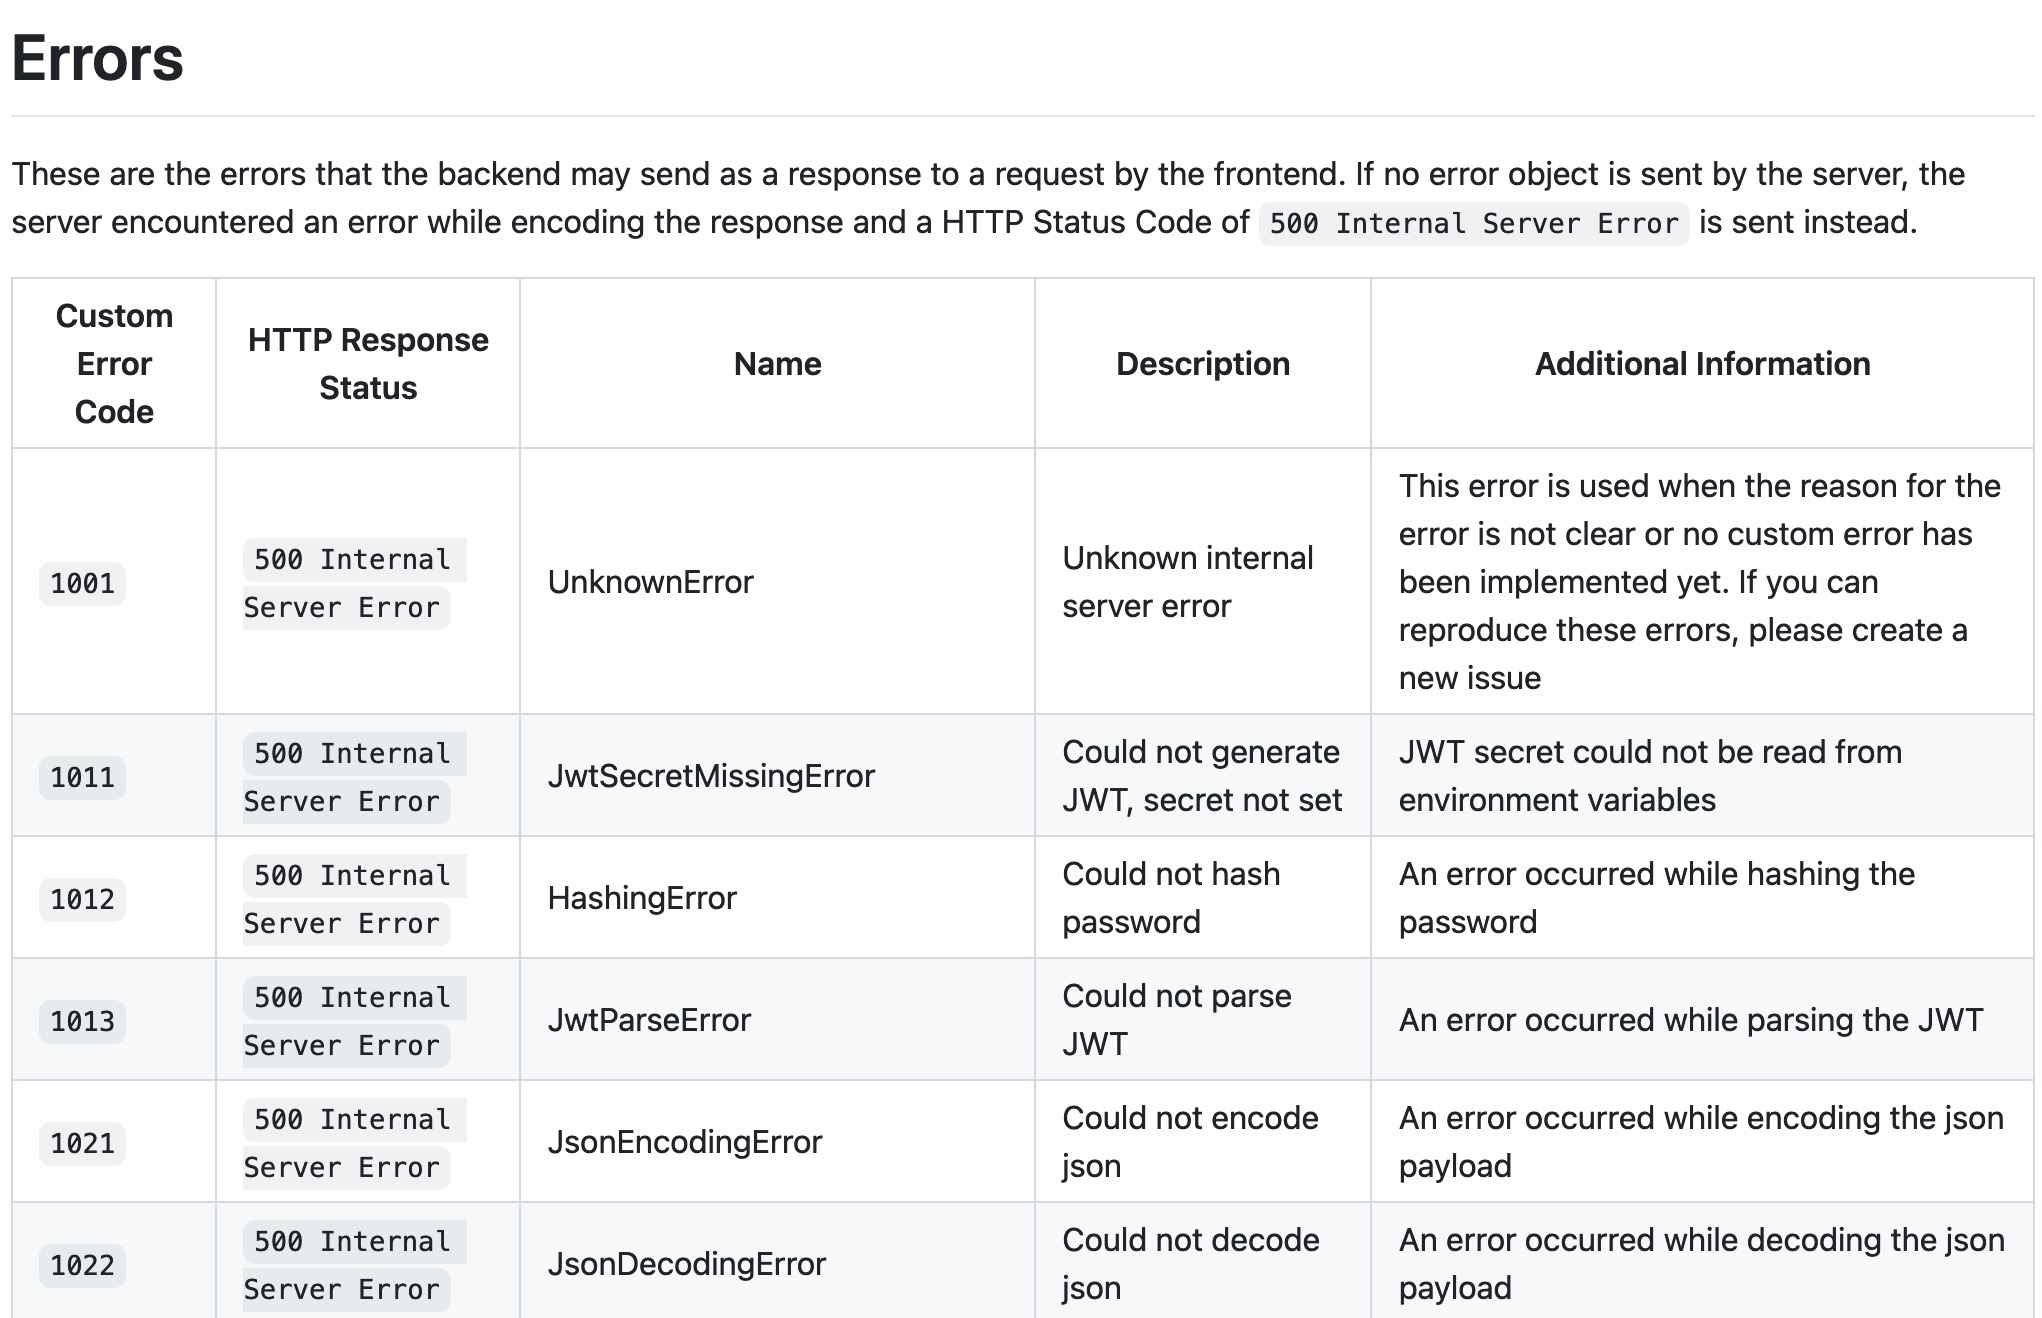
\includegraphics[width=\textwidth]{images/errors_documentation.jpg}
  \caption{Excerpt from the Error Code Documentation for the Backend}
  \label{fig:error_code_documentation}
\end{figure}

\subsubsection{Configuration}
The backend servers are configured through environment variables. These can be
provided in a \texttt{.env} file, which the backend will automatically load on
startup.

The backend implements a system that allows for environment variables to be
optional and for default values to be set. If the backend tries to access a
variable that is only covered by a default value, a warning will be added to the
logs to notify users of potentially unintended configurations (see Line 1 of
Figure \ref{fig:backend_logging}).

Making the backend fully configurable using environment variables makes
deployment and configuration much easier -- especially when compared to
hard-coded values. This is also advantageous during development. Development
environments can vary wildly between developers and this system allows each
developer to have a configuration that fits their needs.

The environment variables were documented during development, no changes were
made without updating the documentation. The readme file for the backend
contained a list of all environment variables (see Figure
\ref{fig:backend_env}).

\begin{figure}[htbp]
  \centering{}
  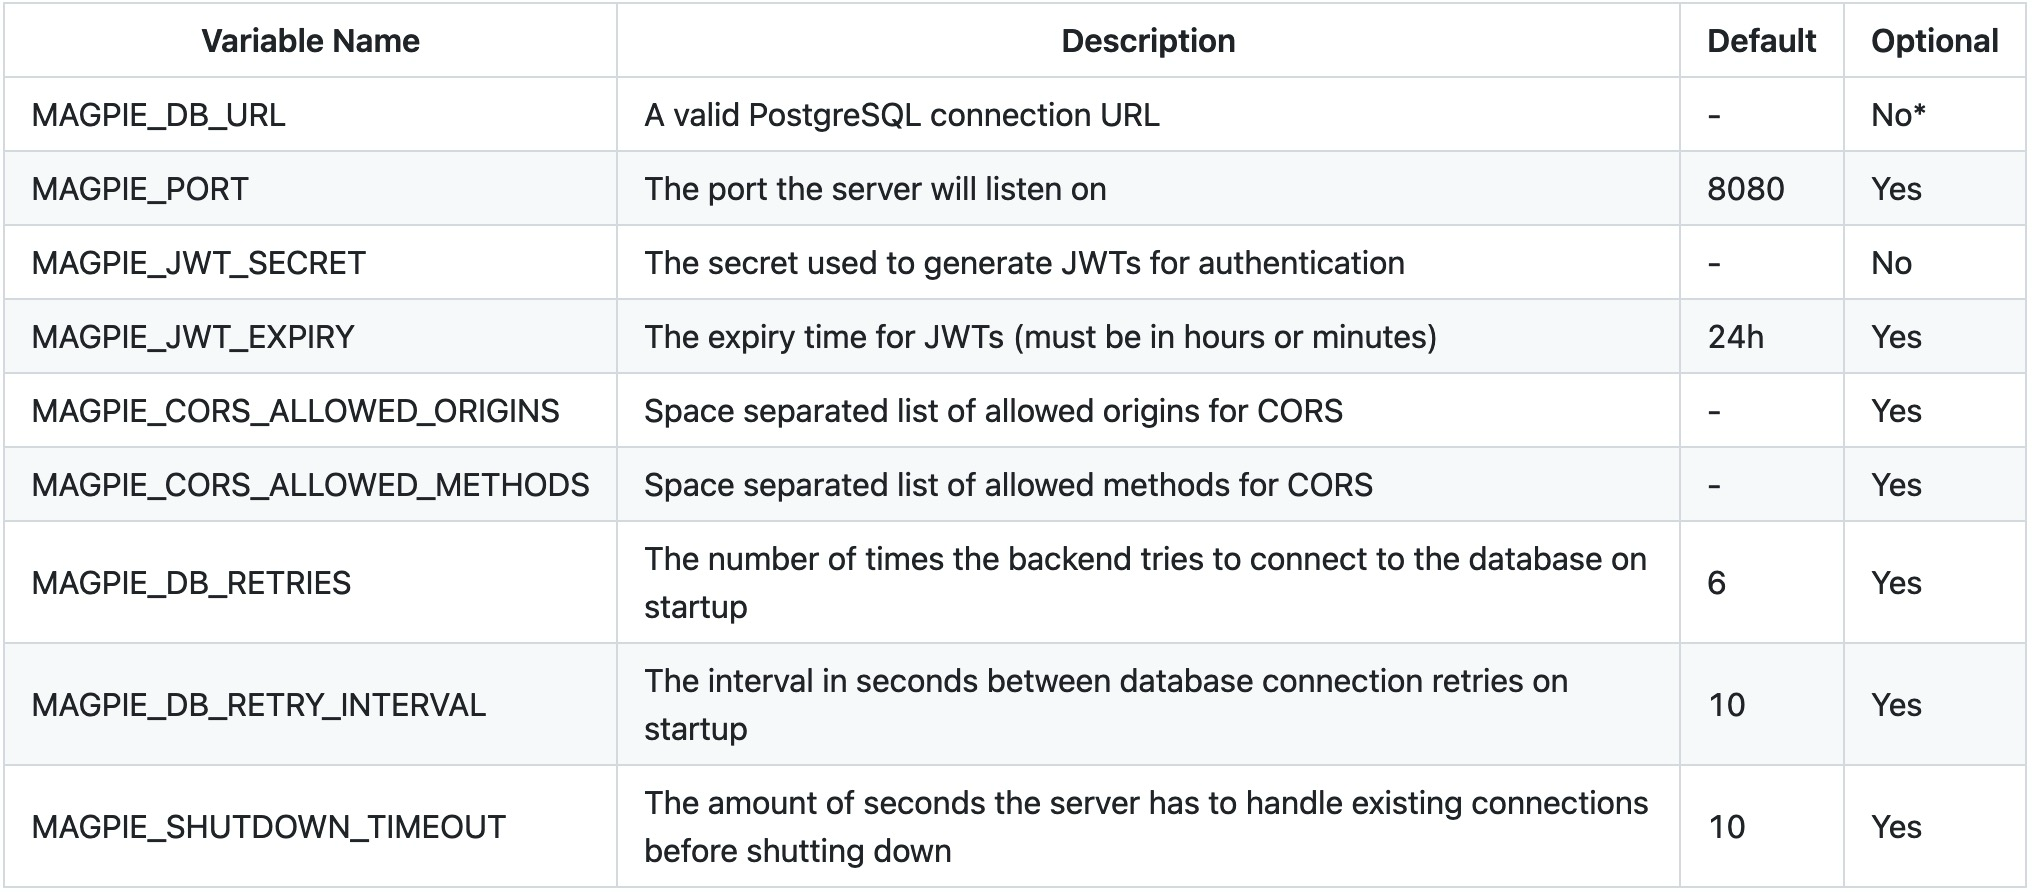
\includegraphics[width=\textwidth]{images/backend_env.png}
  \caption{The environment variables available for configuring the backend}
  \label{fig:backend_env}
\end{figure}

The variable \texttt{MAGPIE\_DB\_URL} can be omitted if the connection information
is instead given as separate environment variables (\texttt{LOGIN},
\texttt{PASSWORD}, \texttt{HOST} and \texttt{DATABASE\_NAME}). This is used for
deployments using Kubernetes. If both \texttt{MAGPIE\_DB\_URL} and the separate
environment variables are set, only \texttt{MAGPIE\_DB\_URL} will be used to
establish a connection.

\subsubsection{Testing}
During development, both backends were outfitted with automated unit testing.
This allowed for bugs to be caught early and consistently. The tests covered all
vital functions of the backends, namely the routing and -- most importantly --
the request handlers.

Implementing unit tests also allows for future regression testing, making it
easier to spot issues like increased latency between versions of the backend.

The test implementation was done using the \texttt{testing} package from the Go
standard library. While there are more advanced alternatives like testify, they
were considered to be too complex for a project of this scope.

In addition to the standard library, \texttt{pgxmock} was used to simulate a
database connection during test execution. This made tests significantly simpler
to set up and implement, as no actual database connection needed to be
maintained for the tests to be effective. Additionally, \texttt{pgxmock}
provides a way to expect certain queries to be executed, which is a valuable
tool for unit tests.

So called table-based tests were used to validate the backends functionality.
For this, a list of inputs (i.e. a table) is defined, which will then be passed
to the function to be tested one by one. Each definition also comes with success
and failure conditions (see Listing \ref{listing:test_case_definition}). Using
this, it is possible to efficiently create a multitude of testcases with
different parameters which share the underlying test execution code.

\newpage{}

\begin{listing}[htbp]
  \centering{}
  \begin{minipage}{0.7\textwidth}
  \begin{minted}{go}
{
  Name: "Valid input",
  Method: "POST",
  Route: "/points",
  InputJSON: `{
    "longlat": {
      "type": "Point",
      "coordinates": [11, 12]
    },
    "type": "parking",
    "details": {
      "test": 1234
    }
  }`,
  MockSetup: func(mock pgxmock.PgxPoolIface) {
    mock.ExpectQuery("INSERT INTO points").
        WithArgs(
          pgxmock.AnyArg(),
          db.PointType("parking"),
          []byte(`{"test":1234}`),
        ).
        WillReturnRows(pgxmock.NewRows([]string{"id"}).
        AddRow(int64(1)))
  },
  ExpectedStatus: http.StatusCreated,
}
  \end{minted}
  \end{minipage}
  \caption{An example of a test case for a table-based unit test of the private points handler}
  \label{listing:test_case_definition}
\end{listing}

To discourage pushing or merging untested code, the decision was made to
automatically run the defined test cases when changes to the backend are pushed
to the repository. For this project, GitHub Actions was used as the CI/CD
solution. At the time of writing this, there is unfortunately no built-in
support for Go unit tests in GitHub Actions.

For this reason, a custom GitHub Action workflow was set up. It automatically
runs the test cases and extracts the test results and code coverage. To make it
easy to check the success of the test cases, the workflow then reports these
metrics as comments on the relevant pull request (see Figures
\ref{fig:backend_github_action} and \ref{fig:backend_github_action_coverage}).
The workflow is configured in a way where any failed tests or insufficient code
coverage lead to the action failing. Since the repository expects all checks to
pass before merging is permitted, this effectively prevents issues to enter the
main code base and by extension the deployment.

\begin{figure}[htbp]
  \centering{}
  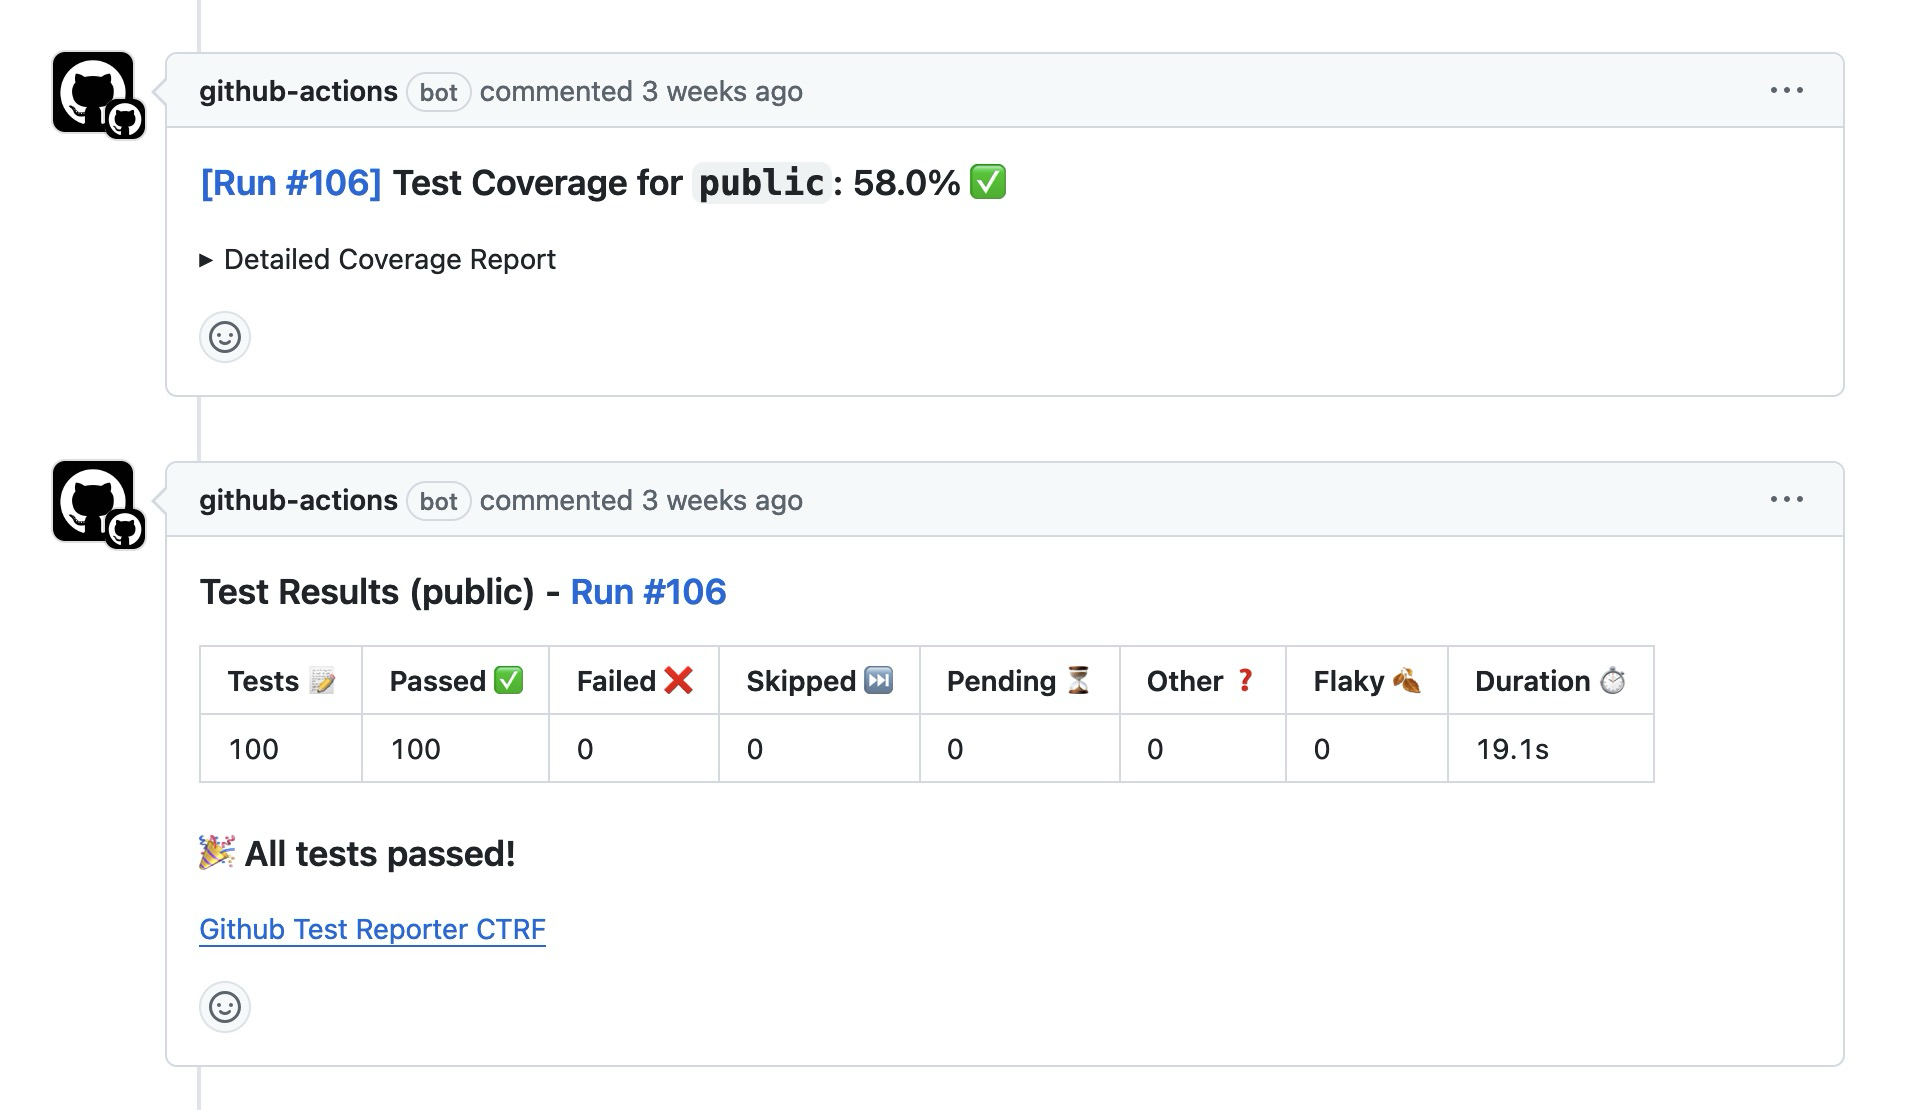
\includegraphics[width=\textwidth]{images/backend_github_action.png}
  \caption{Comments created by custom GitHub action for executing backend unit tests}
  \label{fig:backend_github_action}
\end{figure}

\begin{figure}[htbp]
  \centering{}
  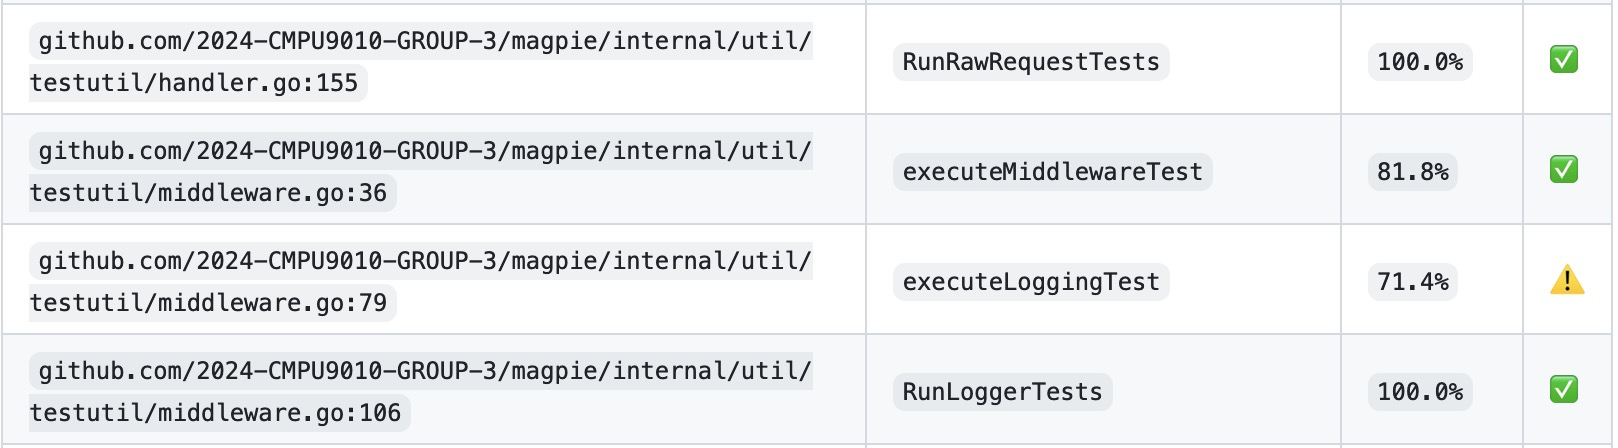
\includegraphics[width=\textwidth]{images/backend_github_action_coverage.png}
  \caption{Excerpt from the hidden section on a coverage comment (see Figure
  \ref{fig:backend_github_action}), providing detailed, function level coverage}
  \label{fig:backend_github_action_coverage}
\end{figure}

\newpage{}